\documentclass[aps,prd,twocolumn,superscriptaddress,nofootinbib,longbibliography,floatfix,showkeys,nobalancelastpage,amsmath,amssymb,10pt]{revtex4-2}
\usepackage[utf8]{inputenc}
\usepackage[T1]{fontenc}
\usepackage{mathptmx}
\usepackage{amsthm}
\usepackage{graphicx}
\usepackage{booktabs}
\usepackage{xcolor}
\usepackage[colorlinks=true,linkcolor=blue!50!black,citecolor=blue!50!black,urlcolor=blue!50!black]{hyperref}
\usepackage{orcidlink}
\usepackage[protrusion=true,expansion=false]{microtype}
\usepackage{xurl}
\makeatletter\let\write@bibliographystyle\relax\let\bibliography@latex\@gobble\makeatother

\theoremstyle{plain}
\newtheorem{theorem}{Theorem}[section]
\newtheorem{proposition}[theorem]{Proposition}
\newtheorem{lemma}[theorem]{Lemma}
\newtheorem{corollary}[theorem]{Corollary}
\theoremstyle{definition}
\newtheorem{definition}[theorem]{Definition}
\newtheorem{remark}[theorem]{Remark}
\theoremstyle{plain}
\newtheorem{mainthm}{Theorem}
\renewcommand{\themainthm}{\Alph{mainthm}}

\newcommand{\NN}{\mathbb{N}}
\newcommand{\eps}{\varepsilon}
\newcommand{\Ex}{\mathcal{E}}
\newcommand{\Tp}{\mathcal{T}}
\newcommand{\Zc}{\mathcal{Z}}
\newcommand{\Jc}{\mathcal{J}}
\newcommand{\Mc}{\mathcal{M}}
\newcommand{\cl}{\mathrm{c}}
\newcommand{\one}{\mathbf{1}}
\newcommand{\repoURL}{https://github.com/creelie/ErdosProblem1}
\tolerance=2000
\emergencystretch=2em
\hbadness=2000
\hfuzz=1pt
\raggedbottom

\begin{document}

\title{An explicit exponent for the exceptional set of the Erd\H{o}s--Straus equation}

\author{Deep Bhattacharjee\,\orcidlink{0000-0003-0466-750X}}
\email{itsdeep@live.com}
\email{d.bhattacharjee@erl-forschung.de}
\thanks{Corresponding author.}
\affiliation{Formerly, Electro-Gravitational Space Propulsion Laboratory (EGSPL), Bhubaneswar, Odisha 751030, India}
\affiliation{Formerly, University of Calcutta, Senate House, 87/1 College Street, Kolkata 700073, West Bengal, India}

\author{Ushashi Bhattacharya\,\orcidlink{0009-0002-2254-3914}}
\email{rai.bhattacharya.in@gmail.com}
\affiliation{Formerly, National Taiwan University, Taipei 106319, Taiwan}

\date{October 19, 2026}

\begin{abstract}
\itshape
The Erd\H{o}s--Straus conjecture says that four divided by any integer greater than one is a sum of three unit fractions. In 1970 Vaughan showed that the integers up to $N$ for which this fails are few: their number is at most $N$ times the exponential of minus a positive constant times the two-thirds power of $\log N$, and his argument gives no value of the constant. We prove this bound with an explicit constant, given by an integral whose value is $0.6792$ and which is at least $0.6657$ in closed form. The residue classes we sieve with include classes to moduli beyond the square root of each prime, which a recent theorem of Maynard lets us count.
\par\medskip\upshape\noindent\textit{2020 Mathematics Subject Classification.} 11D68; 11N36; 11N35; 11N13.
\end{abstract}

\keywords{Erd\H{o}s--Straus conjecture; Egyptian fractions; large sieve; primes in arithmetic progressions}

\maketitle
\makeatletter\renewcommand\l@subsection[2]{}\renewcommand\l@subsubsection[2]{}\makeatother
\tableofcontents

\section{Introduction}\label{sec:intro}

For an integer $n\ge2$ the Erd\H{o}s--Straus conjecture asserts that
\begin{equation}\label{eq:es}
\frac4n=\frac1x+\frac1y+\frac1z
\end{equation}
has a solution in positive integers $x,y,z$ \cite[\S D11]{Guy}. A solution for $n$ gives one for every multiple of $n$, so it is enough to treat primes, and polynomial identities settle every prime outside the six residue classes $1,121,169,289,361,529$ modulo $840$ \cite{Mor}. These six classes are the squares among the classes prime to $840$, and Mordell observed that no identity of this kind can settle a square class.\footnote{An identity that solves \eqref{eq:es} for all $n$ in a class $r$ modulo $q$ exists only if $r$ is not a square modulo $q$; see \cite[Section~2]{ET} for the principle and the families of identities behind it. The same computation decides a recent claim of a proof for the primes $p\equiv1\pmod4$ \cite{Dya}. It reduces the problem to a finite family of classes $p\equiv-4\alpha s^2\pmod{M}$ with $M=4\alpha sr-1$ that is supposed to cover every prime. Since $M\equiv3\pmod4$, $M\equiv-1$ modulo every odd prime factor of $\alpha$, and $M\equiv-1\pmod8$ when $\alpha$ is even, quadratic reciprocity gives the Jacobi symbol $\bigl(\frac{-4\alpha s^2}{M}\bigr)=-1$, so no such class contains a square, and the class $p\equiv1$ modulo $4$ times the product of the moduli is never covered. By Dirichlet's theorem it contains infinitely many primes, all $\equiv1\pmod4$. The reduction is therefore conditional, as its author states.} The conjecture has been verified for all $n\le10^{17}$ by Salez \cite{Sal} and for all $n\le10^{18}$ by Mihnea and Dumitru \cite{MD}. It remains open.

Let $\Ex(N)$ be the set of $n\le N$ for which \eqref{eq:es} has no solution. Vaughan \cite{Vau} proved in 1970 that
\begin{equation}\label{eq:vaughan}
|\Ex(N)|\ll N\exp\bigl(-c(\log N)^{2/3}\bigr)
\end{equation}
for some constant $c>0$, by applying the large sieve to the residue classes produced by one family of identities. Elsholtz and Tao \cite{ET} later determined the average number of solutions of \eqref{eq:es} for prime $n$. Pomerance and Weingartner \cite{PW} extended \eqref{eq:vaughan} to $m/n$ uniformly in $m$, with the exponent $C(\log N)^{2/3}/\varphi(m)^{1/3}$ for an absolute constant $C$. In both papers the number of residue classes at each prime is controlled only up to constant factors, and no numerical value of $c$ follows.\footnote{In \cite[Section~4]{PW} the number of classes, summed over the primes $p\le x$ with weight $1/p$, is shown to be of order $(\log x)^2$: the upper bound comes from the Brun--Titchmarsh inequality and the lower bound from the Bombieri--Vinogradov theorem, with different implied constants, and the exponent is written through these two constants.} Dahan \cite{Dah} has recently run Vaughan's large-sieve scheme on a two-parameter Type~II system for the primes $n\equiv1\pmod{24}$, which contain every prime in $\Ex(N)$, and obtained \eqref{eq:vaughan} for these primes with $c=0.065$. The sum that governs his system has the leading constant $9/(2\pi^2)$, found by Liu \cite{Liu} and, with a power-saving error term, in \cite{BBv1}; with it the same argument gives $c=0.0943$ for the primes. Here we give an explicit constant for the whole set $\Ex(N)$, and we take it beyond the value that the residue classes reachable by the Bombieri--Vinogradov theorem can give.

\begin{mainthm}\label{thm:A}
For every $\eps>0$ there is $N_0(\eps)$ such that, for all $N\ge N_0(\eps)$,
\begin{equation}\label{eq:main}
|\Ex(N)|\le N\exp\bigl(-(c_1-\eps)(\log N)^{2/3}\bigr),
\end{equation}
where
\begin{equation}\label{eq:c1}
c_1=\frac32\Bigl(\frac{9}{8\pi^2}\Bigl(\frac{40}{49}-6\Jc\Bigr)\Bigr)^{1/3}
\end{equation}
and $\Jc$ is the integral \eqref{eq:J} of Section~\ref{sec:strips}. Moreover $0\le\Jc\le533/64680$, so that
\begin{equation}\label{eq:cvar}
c_1\ge c_{\mathrm{var}}=\Bigl(\frac{286983}{98560\,\pi^2}\Bigr)^{1/3}=0.6657102497\ldots
\end{equation}
\end{mainthm}

The number $40/49$ is the share of the triangle of factorisations (Figure~\ref{fig:simplex}) covered by the regions whose residue classes we count, and $6\Jc$ is the part of that share which our count misses. Numerical integration gives $\Jc=0.0003$ and $c_1=0.6792$ (Section~\ref{sec:constant}); two independent programs agree on $c_1$ to four decimals, and a Monte Carlo simulation agrees with the integrand. The lower bound \eqref{eq:cvar} is proved in closed form.

The second theorem concerns the classes that the Bombieri--Vinogradov theorem can count. For a prime $p\equiv3\pmod4$ with $P=(p+1)/4$, let $\Omega^\sharp_p$ be the set of classes $-u/a\pmod p$ attached to factorisations $P=ua\alpha$ with $\gcd(u,a)=1$ in which one of the three products $ua$, $u\alpha$, $a\alpha$ is at most $\sqrt p$ (Section~\ref{sec:typeII}). Let $L^\sharp(Q)$ be the sum that the large sieve attaches to these classes, as in \eqref{eq:L} below.

\begin{mainthm}\label{thm:B}
For every $\eps>0$ there is $N_1(\eps)$ such that, for all $N\ge N_1(\eps)$ and all $Q\ge1$,
\[
\frac{N+Q^2}{L^\sharp(Q)}\ge N\exp\bigl(-(c_0+\eps)(\log N)^{2/3}\bigr),
\]
where
\begin{equation}\label{eq:c0}
c_0=\frac{9}{2^{8/3}\pi^{2/3}}=\frac32\Bigl(\frac{27}{32\pi^2}\Bigr)^{1/3}=0.6607886973\ldots
\end{equation}
\end{mainthm}

The classes $\Omega^\sharp_p$ come from the three corners of the triangle, and with them the large sieve gives exactly the constant $c_0$: Theorem~\ref{thm:B} is the upper bound, and the corners alone already give $c_0$ (Corollary~\ref{cor:density}). The number $27/(32\pi^2)$ inside \eqref{eq:c0} is the density of these classes. The gain from $c_0$ to $c_1$ comes from the classes of the centre of the triangle, which lie beyond the reach of the Bombieri--Vinogradov theorem.

\textit{The method.} Each prime $p\equiv3\pmod4$ carries the identities of Type~II \cite{ET}: for every factorisation $P=ua\alpha$ with $\gcd(u,a)=1$, every $n\equiv-u/a\pmod p$ has a solution of \eqref{eq:es} (Lemma~\ref{lem:identity}). In logarithmic coordinates these factorisations fill a triangle (Figure~\ref{fig:simplex}). To sieve with their classes one must count them over the primes and show that they are distinct. Counting requires primes in progressions to the moduli $4ua$, $4u\alpha$ or $4a\alpha$. The Bombieri--Vinogradov theorem controls such moduli up to about $\sqrt p$, which cuts out three corners of the triangle, where one product of two variables is at most $\sqrt p$. In each corner the class has a normal form of small height, $u/a$, $4u^2\alpha$ or $(4a^2\alpha)^{-1}$, which separates the classes inside that corner, and two arguments with explicit inequalities show that the corner $A$ shares no class with $B$ or $C$. The corners $B$ and $C$ do share classes, but only along a family described by six integers, which contributes a convergent series (Proposition~\ref{prop:BC}). The corners cover three quarters of the triangle and give $c_0$.

The rest of the triangle is the centre, where $u$, $a$ and $\alpha$ are all below $\sqrt P$. There the class $u/a$ is a Farey fraction of order $\sqrt P$, so the classes of the centre are distinct. They differ from the classes of the corners, apart from a family described by five integers, which contains one explicit polynomial family of primes and again contributes a convergent series (Propositions~\ref{prop:centre} and~\ref{prop:centreC}). To count the centre we use a theorem of Maynard \cite{May}: the primes $p\equiv-1\pmod q$ have the expected number for almost all moduli $q$ up to $p^{1/2+\vartheta}$ with $\vartheta<1/42$, provided that $q$ has a divisor in a range that depends on $\vartheta$. A divisor chain (Lemma~\ref{lem:chain}) finds such a divisor for most moduli in three strips of the centre along the corners, and we compute the proportion it misses (Lemma~\ref{lem:density}). If nothing were missed, the strips would add $6(\frac1{84}-\frac3{3528})=\frac{13}{196}$ to the share $\frac34$ of the corners; the loss $6\Jc$ is $0.0018$.

The corners, their normal forms, the treatment of the centre and the rule that finds the divisors were selected by the engine Anaxia of the BLLM project \cite{Ana,BLLM}.\footnote{Anaxia, version~3.0.5, builds constructions by typed crossing of proof components and tests them on data. We ran it twice. On the corners it tested 128 constructions on the $39{,}322$ primes $p\equiv3\pmod4$ below $10^6$ and kept the seven built from one, two or three corners with matching normal forms; the best of them gives $c_0$. On the centre it tested 37 constructions and accepted five, the best of which is the construction of this paper. It rejected the forms $4u^2\alpha$ and $(4a^2\alpha)^{-1}$ in the centre, and a rule that omits the bound on the steps of the divisor chain, by finding counterexamples on data. Section~\ref{sec:verification} describes both runs in full. The engine selected the constructions; the proofs are ours.}

The rest of the argument is analytic. A Rankin-type upper bound and a tilted lower bound determine the sum of the large sieve to leading order once the density of the classes is known (Proposition~\ref{prop:tilt}); the same upper bound proves Theorem~\ref{thm:B}. Section~\ref{sec:constant} computes the constant, Section~\ref{sec:remarks} compares regions of the triangle (Table~\ref{tab:ladder}) and explains where the method stops, and Appendix~\ref{app:derivations} contains every computation in full.

\begin{figure}[t]
\centering
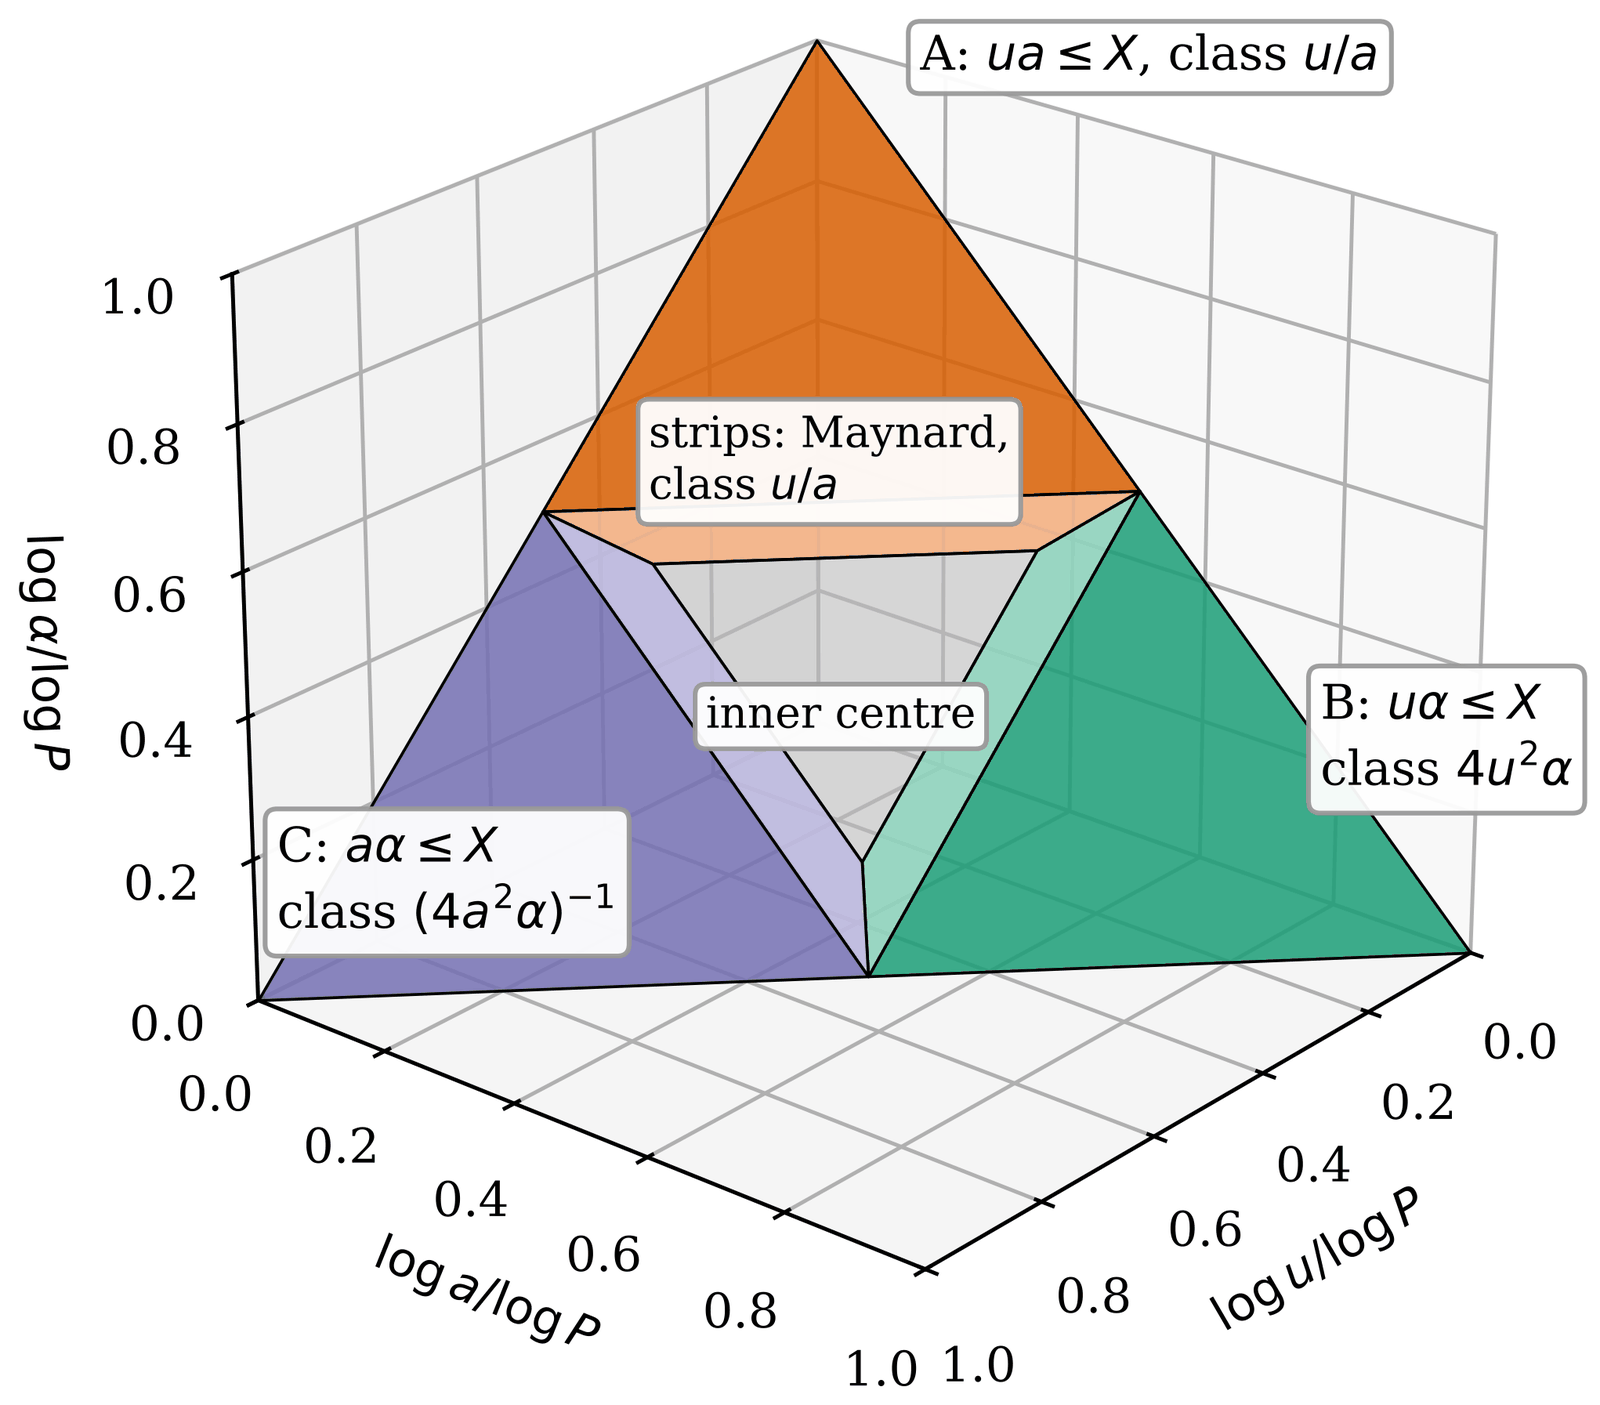
\includegraphics[width=\columnwidth]{figures/fig_simplex.png}
\caption{In the coordinates $(\log u,\log a,\log\alpha)/\log P$ the factorisations $P=ua\alpha$ fill a triangle. The three corners $A$, $B$, $C$ are the parts in which one product of two variables is at most $X$; each carries its own normal form of the class $u/a$ (Lemma~\ref{lem:forms}). At $X=\sqrt p$ each corner has a quarter of the area. In the centre the three coordinates are below $\frac12$ and the class $u/a$ itself separates the classes (Proposition~\ref{prop:centre}). The light strips of the centre along the corners, of depth $\frac1{42}$, are counted with Maynard's theorem (Section~\ref{sec:strips}); they are drawn wider than they are. The inner centre would need moduli beyond Maynard's range.}
\label{fig:simplex}
\end{figure}

\section{Type II triples and their classes}\label{sec:typeII}

Throughout, $p$ denotes a prime with $p\equiv3\pmod4$, and $P=(p+1)/4$, so that $p=4P-1$ and $4P\equiv1\pmod p$.

\begin{definition}\label{def:triple}
A \emph{Type~II triple} for $p$ is $t=(u,a,\alpha)\in\NN^3$ with $ua\alpha=P$ and $\gcd(u,a)=1$. Their set is $\Tp(p)$. The \emph{class} of $t$ is $\cl(t)=u\,a^{-1}\bmod p$, which is defined because $1\le a\le P<p$.
\end{definition}

\begin{lemma}\label{lem:identity}
Let $t=(u,a,\alpha)\in\Tp(p)$ and $n\ge1$ with $n\equiv-\cl(t)\pmod p$. Then $v=(an+u)/p$ is a positive integer and
\begin{equation}\label{eq:identity}
\frac4n=\frac1{\alpha uv}+\frac1{a\alpha nu}+\frac1{a\alpha nv}.
\end{equation}
\end{lemma}

\begin{proof}
The congruence $n\equiv-u/a$ means $p\mid an+u$, and $an+u\ge2$, so $v$ is a positive integer. Then $an+u=pv=(4ua\alpha-1)v$, that is $an+u+v=4a\alpha uv$. Dividing by $a\alpha nuv$ gives \eqref{eq:identity}.
\end{proof}

When $n$ is prime and $n\nmid uv$, two of the three denominators in \eqref{eq:identity} are divisible by $n$ and the third is not; these are the solutions of Type~II in the sense of \cite{ET}.\footnote{The identity \eqref{eq:identity} with $p=4ua\alpha-1$ is the one behind Vaughan's argument \cite{Vau} and the Type~II search of \cite{Dah}; in \cite{BBv1} we used it with $\alpha$ replaced by the witness $s$ of that search.} By Lemma~\ref{lem:identity}, an integer $n\in\Ex(N)$ lies, for every prime $p\equiv3\pmod4$, outside every class $-\cl(t)$ with $t\in\Tp(p)$. This is the input to the large sieve.

\begin{lemma}\label{lem:forms}
For every $t=(u,a,\alpha)\in\Tp(p)$,
\begin{equation}\label{eq:forms}
\cl(t)\equiv4u^2\alpha\equiv(4a^2\alpha)^{-1}\pmod p.
\end{equation}
\end{lemma}

\begin{proof}
From $p=4ua\alpha-1$ we get the identities
\[
4(u^2\alpha)a-u=up,\qquad 4(a^2\alpha)u-a=ap.
\]
The first gives $4u^2\alpha\cdot a\equiv u$, so $u/a\equiv4u^2\alpha$. The second gives $4a^2\alpha\cdot u\equiv a$, so $u/a\equiv(4a^2\alpha)^{-1}$.
\end{proof}

We call $u/a$, $4u^2\alpha$ and $(4a^2\alpha)^{-1}$ the three normal forms of the class. Each is useful where its height is small.

\begin{definition}\label{def:corners}
For $X\ge1$ the three \emph{corners} at level $X$ are
\begin{align*}
A_p(X)&=\{t\in\Tp(p):u\ge2,\ a\ge2,\ ua\le X\},\\
B_p(X)&=\{t\in\Tp(p):u\alpha\le X\},\\
C_p(X)&=\{t\in\Tp(p):a\alpha\le X\}.
\end{align*}
\end{definition}

The corner $A$ omits the triples with $u=1$ or $a=1$, which are needed in the proof of Proposition~\ref{prop:distinct} and are too few to matter in the count (they contribute $O(\log X)$ to the sums of Section~\ref{sec:counting}). The map $\iota(u,a,\alpha)=(a,u,\alpha)$ is an involution of $\Tp(p)$ with $\cl(\iota t)=\cl(t)^{-1}$; it maps $A_p(X)$ onto itself and exchanges $B_p(X)$ and $C_p(X)$. In particular $|B_p(X)|=|C_p(X)|$.

\begin{lemma}\label{lem:geometry}
Suppose $16X^2\le p$. Then:
\begin{enumerate}
\item[(i)] the corners $A_p(X)$, $B_p(X)$, $C_p(X)$ are pairwise disjoint;
\item[(ii)] on $A_p(X)$ one has $u,a\le X$; on $B_p(X)$ one has $u^2\alpha\le X^2$; on $C_p(X)$ one has $a^2\alpha\le X^2$.
\end{enumerate}
\end{lemma}

\begin{proof}
(i) Two of the three conditions force the product of the two products to be at most $X^2$. For $A$ and $B$ this is $(ua)(u\alpha)=uP\le X^2$; for $A$ and $C$ it is $aP\le X^2$; for $B$ and $C$ it is $\alpha P\le X^2$. In each case $P\le X^2\le p/16<P$, which is impossible. (ii) On $A$, $u$ and $a$ divide $ua\le X$. On $B$, $u^2\alpha=u\cdot u\alpha\le(u\alpha)^2\le X^2$, and similarly on $C$.
\end{proof}

\begin{figure}[t]
\centering
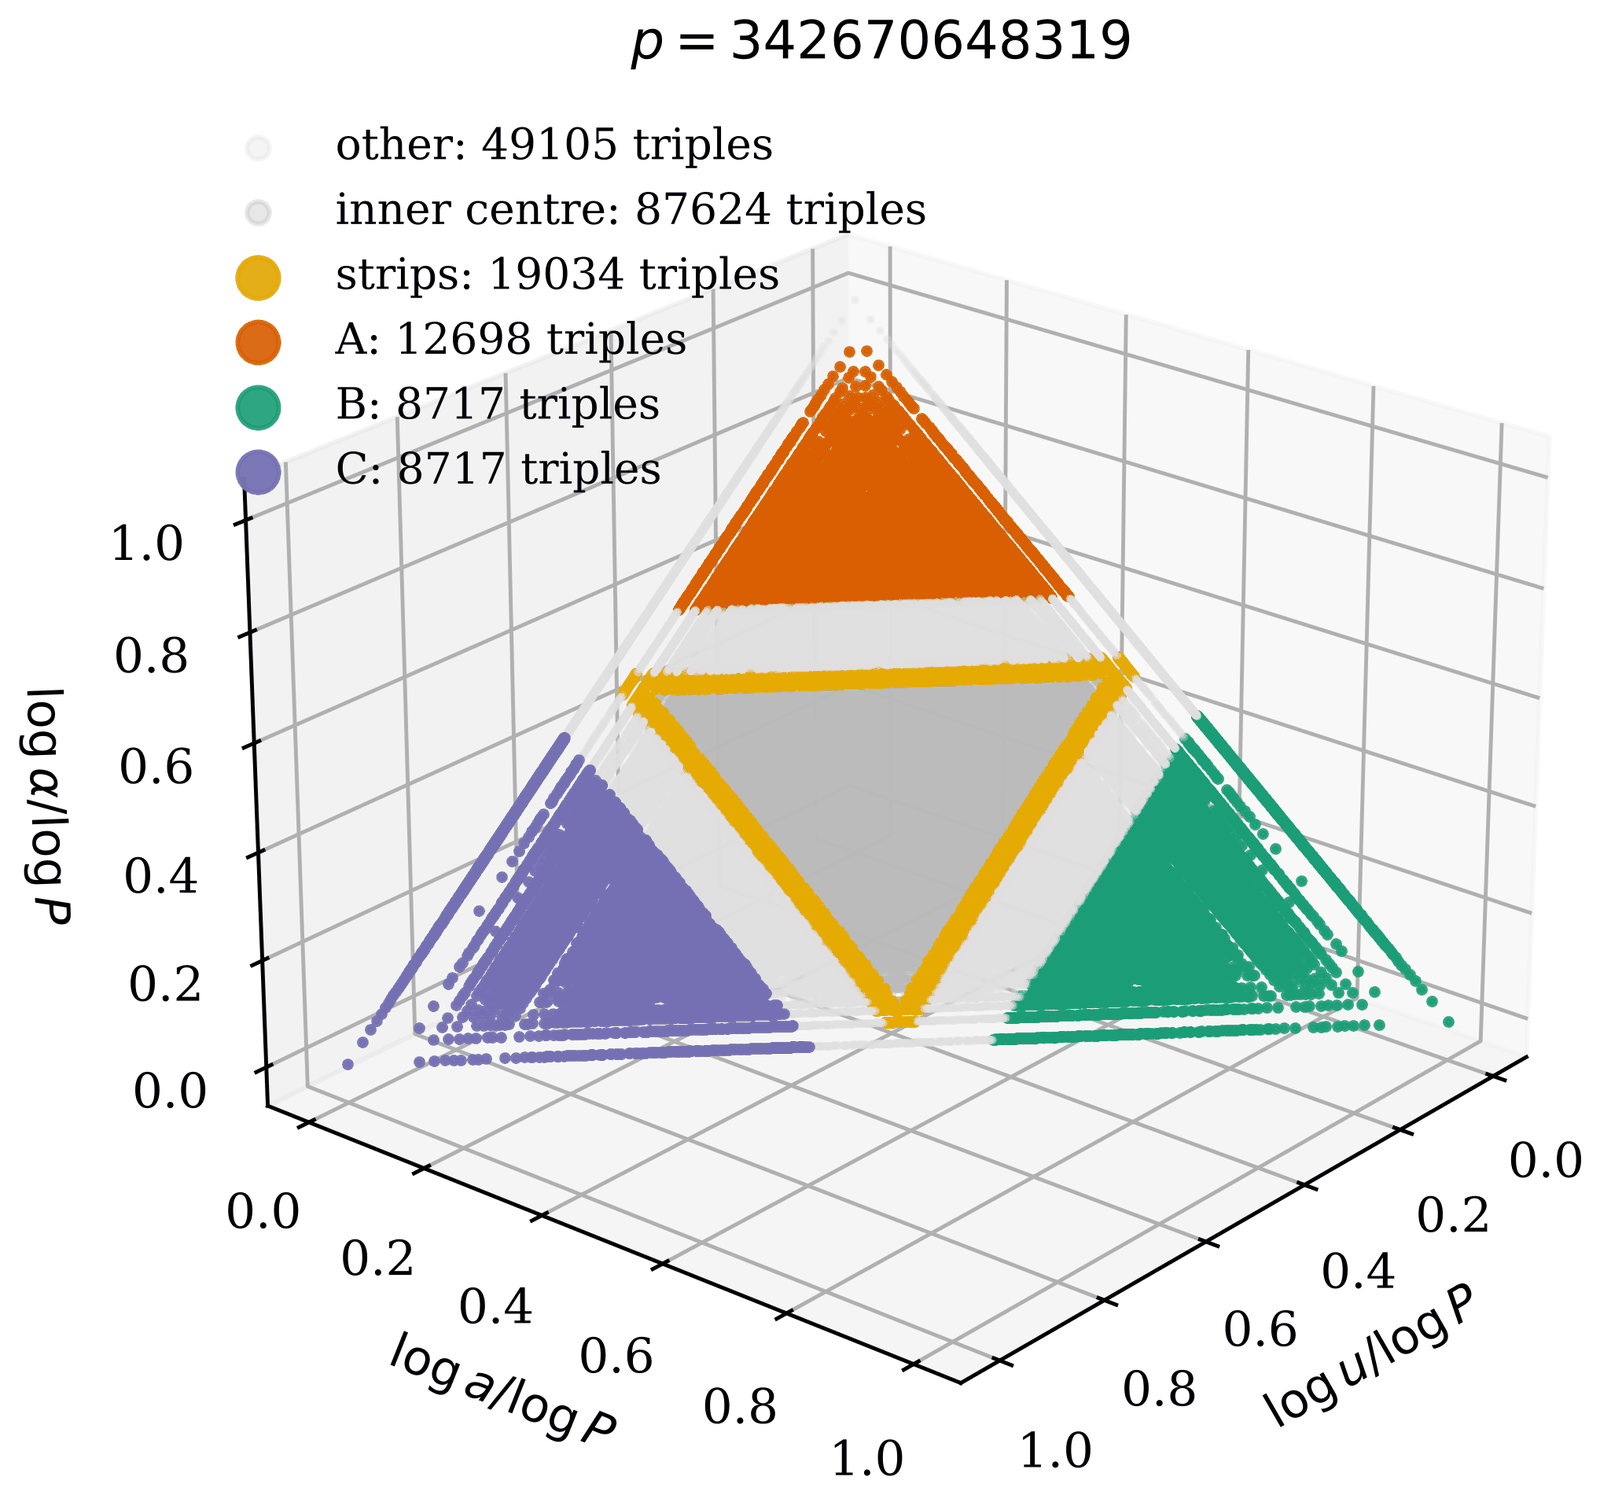
\includegraphics[width=\columnwidth]{figures/fig_triples.png}
\caption{The $185{,}895$ Type~II triples of the prime $p=342670648319$, for which $P=2^8\cdot3^2\cdot5\cdot7\cdot11\cdot13\cdot17\cdot19\cdot23$, with the corners at level $X=\sqrt p/16$, the strips of the centre (largest coordinate at least $P^{1/2-1/42}$) and the inner centre. The light grey triples lie in no corner and outside the centre. The corners $B$ and $C$ have the same size, as the involution $\iota$ shows.}
\label{fig:triples}
\end{figure}

\section{Distinct classes in the corners}\label{sec:distinct}

This section proves that the classes of the three corners are distinct, apart from a sparse set of coincidences between $B$ and $C$.

\begin{proposition}\label{prop:distinct}
Suppose $16X^2\le p$. Then $\cl$ is injective on each of $A_p(X)$, $B_p(X)$ and $C_p(X)$, and no class of $A_p(X)$ is a class of $B_p(X)$ or of $C_p(X)$.
\end{proposition}

\begin{proof}
\emph{Inside $A$.} Let $t,t'\in A_p(X)$ with $u/a\equiv u'/a'$. Then $p\mid ua'-u'a$, and $|ua'-u'a|<X^2<p$ by Lemma~\ref{lem:geometry}(ii), so $ua'=u'a$. Since $\gcd(u,a)=\gcd(u',a')=1$, this gives $u=u'$, $a=a'$ and then $\alpha=\alpha'$.

\emph{Inside $B$.} Let $t,t'\in B_p(X)$ with equal classes. By \eqref{eq:forms}, $4u^2\alpha\equiv4u'^2\alpha'$, and both sides lie in $[1,4X^2]\subset[1,p)$, so $h=u^2\alpha$ equals $h'=u'^2\alpha'$. Now $ha=u\cdot ua\alpha=uP$, so $u/a=h/P$ as rational numbers; since $\gcd(u,a)=1$, the pair $(u,a)$ is the reduced form of $h/P$. The same holds for $t'$, so $t=t'$.

\emph{Inside $C$.} The involution $\iota$ maps $C$ onto $B$ and inverts classes, so injectivity on $C$ follows from injectivity on $B$.

\emph{$A$ against $B$.} Let $t=(u,a,\alpha)\in A_p(X)$ and $t'=(u',a',\alpha')\in B_p(X)$ have the same class, and put $h=u'^2\alpha'$, so that $u/a\equiv4h$ by \eqref{eq:forms}. Then $4ah-u=wp$ for some integer $w$.

If $w\le-1$ then $4ah\le u-p<0$, which is impossible. If $w=0$ then $4ah=u$, so $a\mid u$, and $\gcd(u,a)=1$ forces $a=1$, which is excluded in $A$. Hence $w\ge1$. Substituting $p=4ua\alpha-1$ in $4ah=u+wp$ gives
\[
4ah=u-w+4ua\alpha w,
\]
so $4a\mid u-w$. Write $u-w=4aj$ with $j\in\mathbb{Z}$; then
\begin{equation}\label{eq:hj}
h=j+wu\alpha,\qquad w=u-4aj.
\end{equation}

\emph{Case $j\le-1$.} Then $w=u+4a|j|$ and
\[
h=-|j|+(u+4a|j|)u\alpha=|j|p+u^2\alpha>p,
\]
while $h\le X^2<p$ by Lemma~\ref{lem:geometry}(ii). This is impossible.

\emph{Case $j=0$.} Then $h=u^2\alpha$, and, as in the proof for $B$, $u'/a'=h/P=u^2\alpha/(ua\alpha)=u/a$, so $t'=t$. But $A$ and $B$ are disjoint by Lemma~\ref{lem:geometry}(i).

\emph{Case $j\ge1$.} Since $w\ge1$, \eqref{eq:hj} gives $4aj\le u-1$, so $aj<u/4$. Put $d=u'\alpha'$. Then $P=a'd$ and $h=u'd$, and from \eqref{eq:hj},
\[
a\,h=aj+w\,ua\alpha=aj+wP=aj+wa'd,
\]
that is
\begin{equation}\label{eq:dj}
d\,(au'-a'w)=aj.
\end{equation}
The right side is positive, so $au'-a'w\ge1$ and $d\le aj<u/4$. Hence $h=u'^2\alpha'\le(u'\alpha')^2=d^2<u^2/16$, and
\[
p<u+wp=4ah<\frac{au^2}{4}\le\frac{(ua)^2}{4}\le\frac{X^2}{4}<p,
\]
a contradiction. So no class of $A$ is a class of $B$.

\emph{$A$ against $C$.} If $t\in A_p(X)$ and $t'\in C_p(X)$ had the same class, then $\iota t\in A_p(X)$ and $\iota t'\in B_p(X)$ would have the same class $\cl(t)^{-1}$, which the previous step excludes.
\end{proof}

The corners $B$ and $C$ can share a class. The next proposition describes every such coincidence.

\begin{proposition}\label{prop:BC}
Suppose $16X^2\le p$, and let $t=(u,a,\alpha)\in B_p(X)$ and $t'=(u',a',\alpha')\in C_p(X)$ have the same class. Put
\[
d=u\alpha,\quad e=a'\alpha',\quad M=ua',\quad k=\alpha\alpha',
\]
$G=\gcd(d,e)$, $d=Gd_1$ and $e=Ge_1$. Then there are integers $r,m,\tau\ge1$ such that
\begin{align}
P&=Gd_1e_1(4Gr+\tau),\label{eq:BC-P}\\
M&=d_1e_1\tau(4Gr+\tau)+r,\label{eq:BC-M}\\
G&=4k\tau r+m,\label{eq:BC-G}\\
m(4k\tau r+m)&=k\tau^2+\frac{kr}{d_1e_1},\quad d_1e_1\mid kr,\label{eq:BC-quad}
\end{align}
and
\begin{equation}\label{eq:BC-bounds}
\tau\ge4mr,\qquad G\ge16kmr^2,\qquad P\ge1024\,k^2m^2r^5d_1e_1.
\end{equation}
The integers $k,m,r,d_1,e_1,\tau$ and $u$ determine the pair $(t,t')$.
\end{proposition}

\begin{proof}
\emph{Step 1: the integer $r$.} By \eqref{eq:forms}, $4u^2\alpha\equiv(4a'^2\alpha')^{-1}$, so $16\,u^2\alpha\,a'^2\alpha'\equiv1\equiv16P^2$ and therefore $u^2\alpha\,a'^2\alpha'\equiv P^2$, that is, $de\,M\equiv P^2\pmod p$. On the other hand $P=ad=u'e$, so $P^2=de\cdot au'$. Since $p\nmid de$, we get $au'\equiv M\pmod p$; write $au'=M+rp$ with $r\in\mathbb{Z}$, so that
\begin{equation}\label{eq:BC-r}
P^2=de\,(M+rp).
\end{equation}
If $r=0$ then $au'=ua'$, and since both pairs are coprime, $u=u'$ and $a=a'$, so $t=t'$, which contradicts Lemma~\ref{lem:geometry}(i). If $r\le-1$ then $M=au'+|r|p>p$, but $M=ua'\le(u\alpha)(a'\alpha')\le X^2<p$. Hence $r\ge1$.

\emph{Step 2: the integer $s=P-4der$.} Expanding \eqref{eq:BC-r} with $p=4P-1$ gives
\begin{equation}\label{eq:BC-s}
P\,s=de\,(M-r),\qquad s=P-4der.
\end{equation}
Since $M\ge1$, \eqref{eq:BC-r} gives $P^2>der(4P-1)$, hence $4der<P^2/(P-\frac14)<P+1$, so $s\ge0$. If $s=0$ then $M=r$ and $P=4der$; then $a=P/d=4er=4eua'$, so $u\mid a$ and $u=1$; similarly $u'=P/e=4dr=4dua'$, so $a'\mid u'$ and $a'=1$. Then $r=M=1$ and $P=4de\le4X^2\le p/4<P$, a contradiction. Hence $s\ge1$.

\emph{Step 3: the parametrisation.} Both $d$ and $e$ divide $P$ and $4der$, hence $s$, so the least common multiple $Gd_1e_1$ divides $s$. Write $s=Gd_1e_1\tau$ with $\tau\ge1$. Then $P=s+4der=Gd_1e_1(4Gr+\tau)$, which is \eqref{eq:BC-P}. Inserting this into \eqref{eq:BC-s} and cancelling $G^2d_1e_1$ gives \eqref{eq:BC-M}. Next, $de=ua'\cdot\alpha\alpha'=kM$, so $kM=G^2d_1e_1$. With \eqref{eq:BC-M} this reads $k\,d_1e_1\tau(4Gr+\tau)+kr=G^2d_1e_1$, so $d_1e_1\mid kr$ and
\begin{equation}\label{eq:BC-G2}
G^2-k\tau(4Gr+\tau)=\frac{kr}{d_1e_1}\ge1.
\end{equation}
Hence $G(G-4k\tau r)>k\tau^2>0$, so $m=G-4k\tau r\ge1$, which is \eqref{eq:BC-G}, and \eqref{eq:BC-G2} becomes \eqref{eq:BC-quad}.

\emph{Step 4: the inequalities.} From \eqref{eq:BC-quad}, $4k\tau rm+m^2\le k\tau^2+kr$. Suppose $\tau<4mr$. The integers $\tau$ and $4mr-\tau$ are positive with sum $4mr$, so their product is at least $4mr-1\ge3r\ge r$. Then $k\tau(4mr-\tau)\ge kr$, while the inequality above gives $k\tau(4mr-\tau)\le kr-m^2<kr$. This contradiction proves $\tau\ge4mr$. Then $G=4k\tau r+m\ge16kmr^2$, and from \eqref{eq:BC-P},
\[
P\ge Gd_1e_1\cdot4Gr=4r\,G^2d_1e_1\ge1024\,k^2m^2r^5d_1e_1.
\]

\emph{Step 5: recovery of the pair.} Given $k,m,r,d_1,e_1,\tau$, the integers $G$, $P$, $d$, $e$ and $M$ are fixed by \eqref{eq:BC-G}, \eqref{eq:BC-P} and \eqref{eq:BC-M}. Given also $u$, we recover $\alpha=d/u$, $a'=M/u$, $\alpha'=e/a'$, $a=P/d$ and $u'=P/e$.
\end{proof}

For a prime $p\equiv3\pmod4$ let $\nu(p)$ be the number of pairs $(t,t')$ with $t\in B_p(\sqrt p/4)$, $t'\in C_p(\sqrt p/4)$ and $\cl(t)=\cl(t')$. For every $X\le\sqrt p/4$ the corners at level $X$ lie inside those at level $\sqrt p/4$, so the number of coincidences between $B_p(X)$ and $C_p(X)$ is at most $\nu(p)$.

\begin{corollary}\label{cor:nu}
$\sum_p\nu(p)/p<\infty$.
\end{corollary}

\begin{proof}
Fix $\eta\in(0,\frac14)$. By Proposition~\ref{prop:BC}, each coincidence at $p$ gives integers $k,m,r,d_1,e_1,\tau\ge1$ that fix $P$, together with a divisor $u$ of $M<p$; there are at most $C_\eta P^\eta$ such divisors. For fixed $k,m,r,d_1,e_1$, the equation \eqref{eq:BC-quad} is a quadratic equation in $\tau$ with leading coefficient $k\ne0$, so it has at most two solutions. The pairs $(d_1,e_1)$ with $d_1e_1\mid kr$ number at most $\tau_3(kr)\le C_\eta(kr)^\eta$, where $\tau_3$ counts ordered factorisations into three factors. Using $p>P\ge1024k^2m^2r^5$, we obtain
\[
\sum_p\frac{\nu(p)}{p}\le C'_\eta\sum_{k,m,r\ge1}\frac{(kr)^\eta}{(k^2m^2r^5)^{1-\eta}},
\]
and the series converges because the exponents of $k$, $m$ and $r$ are $2-3\eta$, $2-2\eta$ and $5-6\eta$, all greater than $1$.
\end{proof}

\section{The centre}\label{sec:centre}

\begin{definition}\label{def:centre}
The \emph{centre} of $\Tp(p)$ is
\[
\Zc_p=\{t\in\Tp(p):u^2<P,\ a^2<P,\ \alpha^2<P\}.
\]
\end{definition}

\begin{lemma}\label{lem:centre}
Let $t=(u,a,\alpha)\in\Zc_p$. Then $u,a,\alpha\ge2$, $u\ne a$, and each of the products $ua$, $u\alpha$, $a\alpha$ exceeds $\sqrt P$. In particular $\Zc_p$ is disjoint from the corners at every level $X\le\sqrt p/2$, and $\iota$ maps $\Zc_p$ onto itself.
\end{lemma}

\begin{proof}
Since $a\alpha<\sqrt P\sqrt P=P$, we have $u=P/(a\alpha)>1$, and in the same way $a,\alpha\ge2$. Then $u\ne a$ because $\gcd(u,a)=1$. Next $ua=P/\alpha>P/\sqrt P=\sqrt P$, and in the same way for the other products. Finally $\sqrt P>\sqrt p/2$, and the conditions of the centre are symmetric in $u$ and $a$.
\end{proof}

In the centre the first normal form $u/a$ has numerator and denominator below $\sqrt P$, as for a Farey fraction of order $\sqrt P$, and this separates the classes.

\begin{proposition}\label{prop:centre}
Let $X\le\sqrt p/4$.
\begin{enumerate}
\item[(i)] $\cl$ is injective on $\Zc_p$, and no class of $\Zc_p$ is a class of $A_p(X)$.
\item[(ii)] No class of a triple of $\Zc_p$ with $u<a$ is a class of $B_p(X)$, and no class of a triple of $\Zc_p$ with $u>a$ is a class of $C_p(X)$.
\end{enumerate}
\end{proposition}

\begin{proof}
(i) Let $t,t'\in\Zc_p$ have the same class, so that $p\mid ua'-u'a$. From $u^2<P$ and $a'^2<P$ we get $(ua')^2<P^2$, so $ua'<P$, and in the same way $u'a<P$. Hence $|ua'-u'a|<P<p$, so $ua'=u'a$, and as before $t=t'$. If instead $t'\in A_p(X)$, then $u',a'\le X$ by Lemma~\ref{lem:geometry}(ii), so $ua'$ and $u'a$ are below $\sqrt P\cdot\sqrt p/4<p$; again $ua'=u'a$ and $t=t'$, which contradicts Lemma~\ref{lem:centre}.

(ii) Let $t\in\Zc_p$ with $u<a$. Then $4u^2\alpha<4ua\alpha=p+1$, and $4u^2\alpha\ne p$ because $p$ is odd, so $1\le4u^2\alpha<p$. If $t'\in B_p(X)$ has the same class, then $1\le4u'^2\alpha'\le4X^2<p$ by Lemma~\ref{lem:geometry}(ii), and \eqref{eq:forms} gives $4u^2\alpha=4u'^2\alpha'$. As in the proof of Proposition~\ref{prop:distinct}, both $(u,a)$ and $(u',a')$ are the reduced form of $u^2\alpha/P$, so $t=t'$, which contradicts Lemma~\ref{lem:centre}. The second statement follows by applying $\iota$, which maps the triples of $\Zc_p$ with $u>a$ to those with $u<a$, maps $C_p(X)$ onto $B_p(X)$, and inverts classes.
\end{proof}

The remaining coincidences, between the centre with $u<a$ and the corner $C$ (and their images under $\iota$), have a parametrisation by five integers.

\begin{proposition}\label{prop:centreC}
Let $X\le\sqrt p/4$, and let $t=(u,a,\alpha)\in\Zc_p$ with $u<a$ and $t''=(u'',a'',\alpha'')\in C_p(X)$ have the same class. Put $s=a''\alpha''$. Then there are integers $k,D,j\ge1$ such that
\begin{align}
u''a-ua''&=kp,\label{eq:C0}\\
a&=j+4ks,\label{eq:C1}\\
uD&=sk,\label{eq:C2}\\
\alpha j(j+4ks)&=sa''-D,\label{eq:C3}
\end{align}
and $4ks<a<\sqrt P$. The integers $a''$, $\alpha''$, $k$, $D$ and $j$ determine the pair $(t,t'')$.
\end{proposition}

\begin{proof}
The equality of classes gives $p\mid u''a-ua''$; write $u''a-ua''=kp$. If $k=0$ then $u''a=ua''$ and $t=t''$, which contradicts Lemma~\ref{lem:centre}. If $k\le-1$ then $ua''\ge p+u''a>p$, while $ua''<\sqrt P\cdot X<p$. Hence $k\ge1$. Multiplying \eqref{eq:C0} by $s$ and using $u''s=P$ and $p=4P-1$ gives
\[
P\,(a-4ks)=s\,(ua''-k).
\]
From $k\,(4P-1)<u''a$ we get $ks(4P-1)<Pa<P(4P-1)$, so $ks<P$. If $4ks>a$, the left side is at most $-P<-sk\le s(ua''-k)$, which is impossible. So $j=a-4ks\ge0$. If $j=0$ then $ua''=k$, so $a=4ks=4ua''s$ is a multiple of $u$, and $\gcd(u,a)=1$ forces $u=1$, which contradicts Lemma~\ref{lem:centre}. Hence $j\ge1$, which is \eqref{eq:C1}. Inserting $P=ua\alpha$,
\[
ua\alpha j=s\,(ua''-k),\qquad\text{so}\qquad u\,(sa''-a\alpha j)=sk.
\]
Put $D=sa''-a\alpha j$; then $uD=sk\ge1$, so $D\ge1$, which is \eqref{eq:C2}, and $\alpha ja=sa''-D$ is \eqref{eq:C3}. Finally $a<\sqrt P$ because $t\in\Zc_p$, and $4ks=a-j<a$. Given $a''$, $\alpha''$, $k$, $D$ and $j$, we recover $s=a''\alpha''$, $u=sk/D$, $a=j+4ks$, $\alpha=(sa''-D)/(ja)$, $P=ua\alpha$ and $u''=P/s$.
\end{proof}

For a prime $p\equiv3\pmod4$ let $\nu'(p)$ be the number of pairs $(t,t'')$ with $t\in\Zc_p$, $t''\in B_p(\sqrt p/4)\cup C_p(\sqrt p/4)$ and $\cl(t)=\cl(t'')$.

\begin{corollary}\label{cor:nuprime}
$\sum_p\nu'(p)/p<\infty$.
\end{corollary}

\begin{proof}
By Proposition~\ref{prop:centre}(ii), a pair counted by $\nu'(p)$ has either $u<a$ and $t''\in C_p(\sqrt p/4)$, or $u>a$ and $t''\in B_p(\sqrt p/4)$, and $\iota$ exchanges the two kinds. It is therefore enough to count the first kind. By Proposition~\ref{prop:centreC}, a pair of the first kind at a prime $p\le y$ gives $s=a''\alpha''$ and $k$ with $ks<\sqrt P/4<\sqrt y$, a divisor $D$ of $sk$, and a divisor $j$ of $sa''-D$, which lies in $[1,s^2]\subset[1,y]$. Fix $\eta>0$. For given $(s,k)$ there are at most $\tau(s)\tau(sk)\max_{m\le y}\tau(m)\ll_\eta y^\eta$ choices of $(a'',\alpha'',D,j)$, and the pairs $(s,k)$ with $ks<\sqrt y$ number $O(\sqrt y\log y)$. Hence the pairs of the first kind at the primes $p\le y$ number $O_\eta(y^{1/2+2\eta})$. With $\eta=\frac18$, partial summation gives $\sum_{p\le y}\nu'(p)/p=O(1)$.
\end{proof}

\begin{remark}[A family of coincidences]\label{rem:family}
For an integer $\alpha\ge1$ put
\[
s=16\alpha+1,\quad a=8(8\alpha+1),\quad P=sa\alpha,\quad p=4P-1.
\]
When $p$ is prime, $t=(s,a,\alpha)$ and $t''=(a\alpha,s,1)$ are Type~II triples for $p$ with the same class, since
\[
(a\alpha)\,a-s\cdot s=4P-1=p.
\]
They are coprime pairs because $s$ is odd with $2(8\alpha+1)-s=1$, and $\gcd(s,\alpha)=1$. This is the case $(k,D,j)=(1,1,4)$ of Proposition~\ref{prop:centreC}, with $a''=s$ and $\alpha''=1$. The triple $t$ lies in the centre exactly when $a^2<P$, that is $16\alpha^2-63\alpha-8>0$, that is $\alpha\ge5$, and $t''$ lies in $C_p(\sqrt p/4)$ because $s<16\alpha^{3/2}<\sqrt p/4$. The value $\alpha=5$ gives the prime $p=531359$, with $t=(81,328,5)$ and $t''=(1640,81,1)$:
\[
81^2-328\cdot1640=-531359.
\]
The value $\alpha=7$ gives the prime $p=1442783$, with $t=(113,456,7)$ and $t''=(3192,113,1)$. Together with their images under $\iota$, these four pairs are all the pairs counted by $\nu'(p)$ for the primes $p\equiv3\pmod4$ below $10^7$. Since $p$ is a cubic polynomial in $\alpha$, the family by itself contributes a convergent series to $\sum_p\nu'(p)/p$.
\end{remark}

\section{Counting the classes of the corners}\label{sec:counting}

\subsection{Mean values}

Let $\kappa=9/(2\pi^2)=0.4559453\ldots$, the constant of \cite{Liu,BBv1}. For $X\ge1$ define
\begin{align*}
S_A(X)&=\sum_{\substack{u,a\ge2,\ ua\le X\\ \gcd(u,a)=1}}\frac1{\varphi(4ua)},\\
S_B(X)&=\sum_{u\alpha\le X}\frac{\varphi(u)}{u\,\varphi(4u\alpha)}.
\end{align*}
The weight $1/\varphi(4ua)$ is the density of the primes $p\equiv-1\pmod{4ua}$, that is, of the primes for which $(u,a,\alpha)$ with $\alpha=P/(ua)$ is a triple of $A_p(X)$. In $S_B$ the extra factor $\varphi(u)/u$ is the density of the condition $\gcd(u,a)=1$ among the primes $p\equiv-1\pmod{4u\alpha}$.\footnote{For a prime $q\mid u$, the primes $p\equiv-1\pmod{4u\alpha}$ fall into $q$ classes modulo $4u\alpha q$, all prime to $4u\alpha q$, and $q\mid a=(p+1)/(4u\alpha)$ holds on exactly one of them. By inclusion and exclusion over the prime factors of $u$, the condition $\gcd(u,a)=1$ has density $\prod_{q\mid u}(1-1/q)=\varphi(u)/u$, because $\varphi(4u\alpha q)=q\,\varphi(4u\alpha)$ when $q\mid u$.}

\begin{lemma}\label{lem:mean}
As $X\to\infty$,
\begin{align*}
S_A(X)&=\frac\kappa2\log^2X+O(\log X),\\
S_B(X)&=\frac\kappa2\log^2X+O(\log X).
\end{align*}
\end{lemma}

\begin{proof}[Sketch]
Since $\varphi(4n)=2\varphi(n)$ for odd $n$ and $4\varphi(n)$ for even $n$, we have $1/\varphi(4n)=\psi(n)/(2n)$ with $\psi(n)=\prod_{q\mid n,\,q\text{ odd}}q/(q-1)$. Thus $S_B(X)=\frac12\sum_{u\alpha\le X}W_B(u,\alpha)/(u\alpha)$ with $W_B(u,\alpha)=\psi(u\alpha)\varphi(u)/u$, a function that is multiplicative in the pair. Writing $W_B(u,\alpha)=\sum_{d\mid u,\,e\mid\alpha}g(d,e)$, the function $g$ is supported on $g(1,1)=1$, $g(1,q)=1/(q-1)$ and $g(q,q)=-1/(q-1)$ for odd primes $q$, and $g(2,1)=-\frac12$. Then
\[
S_B(X)=\frac12\sum_{d,e}\frac{g(d,e)}{de}\,H\Bigl(\frac X{de}\Bigr),\qquad H(Y)=\sum_{mn\le Y}\frac1{mn},
\]
and $H(Y)=\frac12\log^2Y+2\gamma\log Y+O(1)$ for $Y\ge1$. The sum $\sum_{d,e}g(d,e)/(de)$ is the Euler product of the local factors $\frac34$ at $2$ and $1+q^{-2}$ at odd $q$, that is $\frac34\cdot\frac{12}{\pi^2}=\frac9{\pi^2}=2\kappa$, and the main term is $\frac12\cdot2\kappa\cdot\frac12\log^2X$. The sum $S_A$ is treated in the same way with $W_A(u,a)=\psi(ua)\one[\gcd(u,a)=1]$; its local factors are again $\frac34$ and $1+q^{-2}$, and the triples with $u=1$ or $a=1$ contribute $O(\log X)$. The details are in Appendices~\ref{app:local} and~\ref{app:hyperbola}.
\end{proof}

The two corners have the same constant because they have the same local factors (Table~\ref{tab:local} in Appendix~\ref{app:local}).

\subsection{Primes}

To count the corners over the primes we use dyadic blocks. Fix $\delta\in(0,\frac1{10}]$. For $j\ge1$ put
\[
I_j=(2^j,2^{j+1}],\qquad X_j=2^{j(1/2-\delta)}.
\]
For $p\in I_j$ we have $16X_j^2\le16\cdot2^{j(1-2\delta)}\le p$ once $j\ge2/\delta$. We write $|K_p(X)|$ for the size of a corner, with the convention $|K_p(X)|=0$ when $p\not\equiv3\pmod4$.

\begin{proposition}\label{prop:primes}
For $K\in\{A,B,C\}$, as $j\to\infty$,
\[
\sum_{p\in I_j}\frac{|K_p(X_j)|}{p}=\frac\kappa2\Bigl(\frac12-\delta\Bigr)^2(\log2)^2\,j+O_\delta\bigl(j^{1/2}\bigr).
\]
\end{proposition}

\begin{proof}
For $C$ the statement is the one for $B$, since $|C_p(X)|=|B_p(X)|$. Let $x=2^{j+1}$ and $z=j^{1/2}$.

\emph{Corner $A$.} A pair $(u,a)$ with $u,a\ge2$, $\gcd(u,a)=1$ and $ua\le X_j$ belongs to $A_p(X_j)$ exactly when $p\equiv-1\pmod{4ua}$. Hence, for $y\in I_j$,
\[
\sum_{2^j<p\le y}|A_p(X_j)|=\sum_{(u,a)}\bigl(\pi(y;4ua,-1)-\pi(2^j;4ua,-1)\bigr).
\]
The moduli $4ua\le4X_j$ are below $x^{1/2}(\log x)^{-B}$ for $j$ large, and each modulus $4n$ arises from at most $\tau(n)$ pairs. The Bombieri--Vinogradov theorem \cite{Bom}, \cite[Chapter~28]{Dav} with these multiplicities (Appendix~\ref{app:bv}) gives
\[
\sum_{2^j<p\le y}|A_p(X_j)|=\bigl(\pi(y)-\pi(2^j)\bigr)S_A(X_j)+O\bigl(x(\log x)^{-3}\bigr)
\]
uniformly in $y\in I_j$.

\emph{Corner $B$.} Let $P_z=\prod_{q\le z}q$. A pair $(u,\alpha)$ with $u\alpha\le X_j$ belongs to $B_p(X_j)$ when $p\equiv-1\pmod{4u\alpha}$ and $\gcd(u,a)=1$, where $a=(p+1)/(4u\alpha)$. For a squarefree $d\mid u$ the condition $d\mid a$ is $p\equiv-1\pmod{4u\alpha d}$. Inclusion and exclusion over the primes $q\le z$ that divide $u$ count the pairs with no common prime factor $q\le z$:
\[
|B^{(z)}_p|=\sum_{u\alpha\le X_j}\ \sum_{d\mid(u,P_z)}\mu(d)\,\one\bigl[p\equiv-1\ (\mathrm{mod}\ 4u\alpha d)\bigr].
\]
These moduli are at most $4X_je^{2z}$, still in the range of the Bombieri--Vinogradov theorem, and a modulus $4n$ arises at most $\tau_3(n)$ times. The main term is $(\pi(y)-\pi(2^j))S_B^{(z)}(X_j)$, where $S_B^{(z)}$ is $S_B$ with $\varphi(u)/u$ replaced by $\prod_{q\mid u,\,q\le z}(1-1/q)$, and $S_B\le S_B^{(z)}\le S_B+O(\log^2X_j/z)$ (Appendix~\ref{app:large}). Then $|B_p(X_j)|\le|B^{(z)}_p|$, and the difference counts pairs with $q\mid u$ and $q\mid a$ for some prime $q>z$. The Brun--Titchmarsh inequality \cite{MV} bounds their total over $p\in I_j$ by $O(\delta^{-1}\pi(I_j)\log^2X_j/z)$ (Appendix~\ref{app:large}).

\emph{The weights $1/p$.} Partial summation inside the block (Appendix~\ref{app:block}) turns the counts into
\[
\sum_{p\in I_j}\frac{|K_p(X_j)|}{p}=S_K(X_j)\sum_{p\in I_j}\frac1p+O\Bigl(\frac{j}{\delta z}\Bigr)+O(1),
\]
with $S_C=S_B$. By the prime number theorem with error term, $\sum_{p\in I_j}1/p=1/j+O(1/j^2)$. With $S_K(X_j)=\frac\kappa2(\frac12-\delta)^2(\log2)^2j^2+O(j)$ from Lemma~\ref{lem:mean} and $z=j^{1/2}$, this is the statement.
\end{proof}

For $p\in I_j$ with $j\ge2/\delta$ let $\omega^{\mathrm{cor}}_\delta(p)$ be the number of distinct classes $-\cl(t)$ with $t$ in one of the three corners at level $X_j$, and let $\omega^{\mathrm{cor}}_\delta(p)=0$ for all other primes. For a function $\omega$ on the primes define
\begin{equation}\label{eq:N}
N[\omega](\lambda)=\sum_{p\le e^\lambda}\frac{\omega(p)}p.
\end{equation}

\begin{corollary}\label{cor:density}
As $\lambda\to\infty$, $N[\omega^{\mathrm{cor}}_\delta](\lambda)=(a^{\mathrm{cor}}_\delta+o(1))\lambda^2$ with
\[
a^{\mathrm{cor}}_\delta=\frac{3\kappa}4\Bigl(\frac12-\delta\Bigr)^2.
\]
In particular $a^{\mathrm{cor}}_\delta\to a_0=3\kappa/16=27/(32\pi^2)$ as $\delta\to0$.
\end{corollary}

\begin{proof}
By Propositions~\ref{prop:distinct} and~\ref{prop:BC},
\[
\sum_K|K_p(X_j)|-\nu(p)\le\omega^{\mathrm{cor}}_\delta(p)\le\sum_K|K_p(X_j)|.
\]
Summing Proposition~\ref{prop:primes} over the three corners and over $2/\delta\le j\le J$ gives
\begin{align*}
\frac{3\kappa}2\Bigl(\frac12-\delta\Bigr)^2&(\log2)^2\sum_{j\le J}j+O_\delta(J^{3/2})\\
&=a^{\mathrm{cor}}_\delta(J\log2)^2+O_\delta(J^{3/2}).
\end{align*}
The coincidences contribute $O(1)$ by Corollary~\ref{cor:nu}, and a partial block contributes $O(J)$. With $J\log2=\lambda+O(1)$ the corollary follows.
\end{proof}

\section{The strips of the centre}\label{sec:strips}

\subsection{Maynard's theorem}

For $0<\vartheta<\frac1{42}$ put
\begin{equation}\label{eq:theta}
\theta(\vartheta)=\min\Bigl(\frac1{10}-\frac{7\vartheta}5,\ \frac12-19\vartheta\Bigr).
\end{equation}

\begin{theorem}[Maynard {\cite[Corollary~1.2]{May}}]\label{thm:maynard}
Let $b\in\mathbb Z$, $0<\vartheta<\frac1{42}$ and $0<\eta<(1-42\vartheta)/4$, and let $Q_{\vartheta,\eta}(y)$ be the set of $q\le y^{1/2+\vartheta}$ that have a divisor $d$ with $y^{2\vartheta+\eta}<d<y^{\theta(\vartheta)-\eta}$. Then for every $A>0$,
\[
\sum_{\substack{q\in Q_{\vartheta,\eta}(y)\\(q,b)=1}}\Bigl|\pi(y;q,b)-\frac{\pi(y)}{\varphi(q)}\Bigr|\ll_{b,\eta,A}\frac y{(\log y)^A}.
\]
\end{theorem}

We use it with $b=-1$, so that every $q$ is prime to $b$.\footnote{The range $(y^{2\vartheta},y^{\theta(\vartheta)})$ for the divisor is not empty exactly when $\vartheta<\frac1{42}$, and its upper end is $y^{1/10-7\vartheta/5}$ exactly when $\vartheta\le\frac1{44}$. Its width is at least its lower end, $\theta(\vartheta)-2\vartheta\ge2\vartheta$, exactly when $\vartheta\le\frac1{54}$. These three values are where the integrand of \eqref{eq:J} changes its shape (Figure~\ref{fig:strips}).} The theorem asks for a divisor of the modulus in a prescribed range. For the moduli $4ua$ of the centre, the next lemma finds one from the factorisations of $u$ and $a$.

\subsection{A divisor in a window}

\begin{definition}\label{def:rule}
Let $1<A<B$ and $G=\min(B/A,A)$. For $n\ge1$ let $T(n)$ be the product of the prime powers $q^e\parallel n$ with $q<G$, and let $q(n)$ be the largest prime factor of $n$ in $[G,A]$, or $q(n)=1$ if there is none. A pair $(u,v)$ of positive integers \emph{passes the rule} for the window $(A,B)$ if
\begin{enumerate}
\item[(R1)] $u\in(A,B)$ or $v\in(A,B)$; or
\item[(R2)] $uv$ has a prime factor in $(A,B)$; or
\item[(R3)] $q(uv)\,T(uv)>A$.
\end{enumerate}
\end{definition}

\begin{lemma}\label{lem:chain}
If $(u,v)$ passes the rule for $(A,B)$, then $uv$ has a divisor in $(A,B)$.
\end{lemma}

\begin{proof}
Under (R1) or (R2) this is clear. Suppose (R3) holds, and let $r_1,\dots,r_m$ be the prime factors of $T(uv)$, listed with multiplicity; each is below $G$. Put $d_0=q(uv)$ and $d_i=d_0r_1\cdots r_i$. Since $q(uv)\ge G$ when it is a prime, $d_0$ is prime to $T(uv)$, so every $d_i$ divides $uv$. Now $d_0\le A<d_m$, so there is a least $i\ge1$ with $d_i>A$, and then
\[
d_i=d_{i-1}r_i<A\,G\le A\cdot\frac BA=B.
\]
So $d_i$ is a divisor of $uv$ in $(A,B)$.
\end{proof}

The bound $r_i<G\le B/A$ on the steps of the chain is needed.\footnote{If $T(n)$ collected all the prime factors below $A$, the integer $4$ and the window $(\frac52,\frac72)$ would pass (R3) with $T(4)=4>\frac52$, while none of the divisors $1$, $2$, $4$ lies in the window. A brute-force check finds this failure $12{,}022{,}742$ times among the integers up to $2\cdot10^6$ and 64 windows, and no failure of Lemma~\ref{lem:chain} (Section~\ref{sec:verification}).} The condition $G\le A$ keeps the primes of $T(uv)$ apart from $q(uv)$.

\subsection{The density of the pairs that fail}

Let $0<\theta^-<\theta^+$ and put $\xi=\min(\theta^+-\theta^-,\theta^-)$. For a window $(x^{\theta^-},x^{\theta^+})$ the number $G$ of Definition~\ref{def:rule} is $x^\xi$. For $w\ge\xi$ let
\[
\mathcal A_w=(\xi,w]\cup[\theta^+,\infty),
\]
and let $\varpi_w$ be the function on $\mathbb R$ that vanishes on $(-\infty,\xi]$ and satisfies
\begin{equation}\label{eq:varpi}
r\,\varpi_w(r)=\one_{\mathcal A_w}(r)+\int_{\mathcal A_w\cap(0,r)}\varpi_w(r-z)\,dz\qquad(r>\xi).
\end{equation}
The right side involves $\varpi_w$ only on $(-\infty,r-\xi)$, so \eqref{eq:varpi} determines $\varpi_w$ on $(\xi,2\xi]$, then on $(2\xi,3\xi]$, and so on. Let $\rho$ be Dickman's function, with $\rho(v)=1$ for $0\le v\le1$ and $v\rho'(v)=-\rho(v-1)$ for $v>1$. For $s_1,s_2>\theta^-$ put $U(s_1,s_2)=0$ if $s_1$ or $s_2$ lies in $(\theta^-,\theta^+)$, and otherwise
\begin{equation}\label{eq:U}
U(s_1,s_2)=\iint_{\Delta}\rho(t_1/\xi)\rho(t_2/\xi)\varpi_w(s_1-t_1)\varpi_w(s_2-t_2)\,dt_1dt_2,
\end{equation}
where $\Delta=\{t_1,t_2\ge0,\ t_1+t_2\le\theta^-\}$ and $w=\max(\theta^--t_1-t_2,\xi)$. Then $0\le U\le1$ (Appendix~\ref{app:density}).

The function $U$ is the density of the pairs that fail the rule. A number $u$ of size $x^{s_1}$ splits as $u=T(u)\,r$, where the $x^\xi$-smooth part $T(u)$ has size $x^{t_1}$ with density $\rho(t_1/\xi)$, and the rough part $r$ has prime factors $x^{z_i}$ with $z_i\ge\xi$, distributed with density $\prod_idz_i/z_i$ by Mertens' theorem.\footnote{For a number counted with the weight $1/n$ the logarithmic sizes of its prime factors above $x^\xi$ behave like the points of a Poisson process with intensity $dz/z$ on $[\xi,\infty)$, and its $x^\xi$-smooth part is independent of them; this is the content of the theorems of Mertens and of Dickman and de Bruijn \cite[Chapter~III.5]{Ten}. Equation \eqref{eq:varpi} is the renewal equation for the density of $\sum_iz_i$ when every $z_i$ is restricted to $\mathcal A_w$; with $\mathcal A_w$ replaced by $(\xi,\infty)$ it is Buchstab's equation.} The pair fails (R1) and (R2) when $s_1,s_2\notin(\theta^-,\theta^+)$ and no $z_i$ lies in $(\theta^-,\theta^+)$, and it fails (R3) when $t_1+t_2\le\theta^-$ and every $z_i$ in $[\xi,\theta^-]$ is at most $\theta^--t_1-t_2$. These conditions say that all the $z_i$ lie in $\mathcal A_w$.

\begin{lemma}\label{lem:density}
Let $0<\theta^-<\theta^+$, let $U$ be the function \eqref{eq:U}, and let $R\subset(\theta^-,K)^2$, for some $K$, be a set whose boundary has Lebesgue measure zero. Let $h:\NN^2\to\mathbb R$ satisfy $\sum_{d,e}|h(d,e)|/(de)<\infty$, and put
\[
W(u,v)=\sum_{d\mid u,\,e\mid v}h(d,e),\qquad H=\sum_{d,e}\frac{h(d,e)}{de}.
\]
Then, as $x\to\infty$,
\begin{align*}
\sum_{(u,v)}\frac{W(u,v)}{uv}&=H(\log x)^2\iint_R(1-U)\,ds_1\,ds_2\\
&\quad+o\bigl((\log x)^2\bigr),
\end{align*}
where $(u,v)$ runs over the pairs that pass the rule for $(x^{\theta^-},x^{\theta^+})$ and satisfy $(\log u,\log v)/\log x\in R$.
\end{lemma}

The proof is in Appendix~\ref{app:density}.

\subsection{The pieces}

Fix $\delta\in(0,\frac1{200}]$ and a partition
\[
\delta=\vartheta_0<\vartheta_1<\dots<\vartheta_m=\frac1{42}-2\delta,\qquad\vartheta_{i+1}-\vartheta_i\le\delta.
\]
For $0\le i<m$ put
\[
\vartheta_i^+=\vartheta_{i+1}+\delta,\qquad\theta_i^-=2\vartheta_i^++\delta,\qquad\theta_i^+=\theta(\vartheta_i^+)-\delta.
\]
Since $\vartheta_i^+\le\frac1{42}-\delta$, we have $\frac1{10}-\frac{17}5\vartheta_i^+\ge\frac2{105}$ and $\frac12-21\vartheta_i^+\ge21\delta$, so $\theta_i^+-\theta_i^-=\theta(\vartheta_i^+)-2\vartheta_i^+-2\delta>0$. As before, $x=2^j$ for the block $I_j=(x,2x]$.

\begin{definition}\label{def:pieces}
For a prime $p\equiv3\pmod4$ in $I_j$ and $0\le i<m$, let $\Zc^A_{p,i}$ be the set of triples $t=(u,a,\alpha)\in\Tp(p)$ with
\[
x^{1/2+\vartheta_i}<ua\le x^{1/2+\vartheta_{i+1}},\qquad u,a>x^{\theta_i^-},
\]
such that $(u,a)$ passes the rule for the window $(x^{\theta_i^-},x^{\theta_i^+})$. Let $\Zc^B_{p,i}$ be defined in the same way with the pair $(u,\alpha)$ in place of $(u,a)$, and let $\Zc^C_{p,i}=\iota(\Zc^B_{p,i})$, defined with the pair $(a,\alpha)$.
\end{definition}

\begin{lemma}\label{lem:pieces}
Let $j$ be large in terms of $\delta$ and $p\in I_j$. Then every piece $\Zc^K_{p,i}$ lies in the centre $\Zc_p$. In $\Zc^A_{p,i}$ the largest coordinate is $\alpha$, in $\Zc^B_{p,i}$ it is $a$, and in $\Zc^C_{p,i}$ it is $u$. The pieces $\Zc^K_{p,i}$, for $K\in\{A,B,C\}$ and $0\le i<m$, are pairwise disjoint.
\end{lemma}

\begin{proof}
Let $t\in\Zc^A_{p,i}$. Since $x<p\le2x$ we have $x/4<P<x$. Since $\theta_i^-=2\vartheta_{i+1}+3\delta$,
\[
u=\frac{ua}a<x^{1/2+\vartheta_{i+1}-\theta_i^-}=x^{1/2-\vartheta_{i+1}-3\delta},
\]
so $u^2<x^{1-8\delta}<x/4<P$ for $j$ large, and in the same way $a^2<P$. Next $\alpha=P/(ua)<Px^{-1/2}$, so $\alpha^2<P\cdot P/x<P$. Hence $t\in\Zc_p$. Moreover $\alpha\ge P/x^{1/2+\vartheta_{i+1}}>\frac14x^{1/2-\vartheta_{i+1}}$, which exceeds $u$ and $a$ for $j$ large. The pieces $\Zc^B_{p,i}$ and $\Zc^C_{p,i}$ are treated in the same way. Pieces with different $K$ are disjoint because their largest coordinates differ, and pieces with the same $K$ and different $i$ are disjoint because the ranges of the relevant product are disjoint.
\end{proof}

\begin{proposition}\label{prop:strips}
For $K\in\{A,B,C\}$ and $0\le i<m$, as $j\to\infty$,
\[
\sum_{p\in I_j}\frac{|\Zc^K_{p,i}|}p=\kappa(\log2)^2\,\Mc_i\,j+o(j),
\]
where $\Mc_i=\iint_{R_i}(1-U_i)\,ds_1\,ds_2$, with
\[
R_i=\Bigl\{(s_1,s_2):\tfrac12+\vartheta_i<s_1+s_2\le\tfrac12+\vartheta_{i+1},\ s_1,s_2>\theta_i^-\Bigr\}
\]
and $U_i$ the function \eqref{eq:U} for the window $(\theta_i^-,\theta_i^+)$.
\end{proposition}

\begin{proof}
For $C$ the statement is the one for $B$, since $\iota$ is a bijection from $\Zc^B_{p,i}$ onto $\Zc^C_{p,i}$. Write $\eta=\delta/2$.

\emph{The moduli are in Maynard's range.} Let $(u,a)$ satisfy the conditions of Definition~\ref{def:pieces} and let $y\in[x,2x]$. The modulus $q=4ua$ satisfies $q\le4x^{1/2+\vartheta_{i+1}}\le y^{1/2+\vartheta_i^+}$ for $j$ large. By Lemma~\ref{lem:chain}, $ua$ has a divisor $d$ with $x^{\theta_i^-}<d<x^{\theta_i^+}$, and for $j$ large
\[
y^{2\vartheta_i^++\eta}<x^{\theta_i^-},\qquad x^{\theta_i^+}<y^{\theta(\vartheta_i^+)-\eta}.
\]
Since $1-42\vartheta_i^+\ge42\delta$, we have $\eta<(1-42\vartheta_i^+)/4$. Hence $q\in Q_{\vartheta_i^+,\eta}(y)$.

\emph{The piece $A$.} A coprime pair $(u,a)$ as above gives a triple of $\Zc^A_{p,i}$ exactly when $p\equiv-1\pmod{4ua}$, and each modulus $4n$ arises from at most $\tau(n)$ pairs. Theorem~\ref{thm:maynard} with these multiplicities, applied at the points $y_l=x(1+l/j)$ for $0\le l\le j$, and partial summation over the subintervals $(y_l,y_{l+1}]$ (Appendix~\ref{app:maynard}) give
\[
\sum_{p\in I_j}\frac{|\Zc^A_{p,i}|}p=\Bigl(\sum_{p\in I_j}\frac1p\Bigr)\sum_{(u,a)}\frac1{\varphi(4ua)}+O(1),
\]
where $(u,a)$ runs over the coprime pairs that pass the rule with $(\log u,\log a)/\log x\in R_i$. By \eqref{eq:phi4n}, $1/\varphi(4ua)=W_A(u,a)/(2ua)$ with $W_A(u,a)=\psi(ua)\one[\gcd(u,a)=1]$, which has the form of Lemma~\ref{lem:density} with $H=2\kappa$ (Appendix~\ref{app:local}). Lemma~\ref{lem:density} gives $\sum_{(u,a)}1/\varphi(4ua)=\kappa(j\log2)^2\Mc_i+o(j^2)$, and $\sum_{p\in I_j}1/p=1/j+O(1/j^2)$.

\emph{The piece $B$.} A pair $(u,\alpha)$ gives a triple of $\Zc^B_{p,i}$ when $p\equiv-1\pmod{4u\alpha}$ and $\gcd(u,a)=1$ with $a=(p+1)/(4u\alpha)$. As in Proposition~\ref{prop:primes}, inclusion and exclusion over $d\mid(u,P_z)$ with $z=j^{1/2}$ replaces this by the progressions modulo $4u\alpha d$. These moduli are at most $4x^{1/2+\vartheta_{i+1}}e^{2z}\le y^{1/2+\vartheta_i^+}$ and keep the divisor of $u\alpha$ found by Lemma~\ref{lem:chain}, so they lie in $Q_{\vartheta_i^+,\eta}(y)$, and a modulus $4n$ arises from at most $\tau_3(n)$ triples $(u,\alpha,d)$. The main term carries the weight $\psi(u\alpha)\prod_{q\mid u,\,q\le z}(1-1/q)$, which differs from $W_B(u,\alpha)=\psi(u\alpha)\varphi(u)/u$ by a total of $O(j^2/z)$ over the piece (Appendix~\ref{app:large}), and $W_B$ has $H=2\kappa$. The pairs with a common prime factor $q>z$ of $u$ and $a$ contribute $O(j/z)+o(1)$ (Appendix~\ref{app:Blarge}). The rest is as for $A$.
\end{proof}

\subsection{The density of all the classes}

For $p\in I_j$ with $j$ large in terms of $\delta$, let $\omega_\delta(p)$ be the number of distinct classes $-\cl(t)$ with $t$ in one of the three corners at level $X_j$ or in one of the pieces $\Zc^K_{p,i}$, and let $\omega_\delta(p)=0$ for all other primes.

\begin{corollary}\label{cor:combined}
As $\lambda\to\infty$, $N[\omega_\delta](\lambda)=(a_\delta+o(1))\lambda^2$ with
\[
a_\delta=\frac{3\kappa}4\Bigl(\frac12-\delta\Bigr)^2+\frac{3\kappa}2\sum_{i<m}\Mc_i.
\]
\end{corollary}

\begin{proof}
The corners at level $X_j\le\sqrt p/4$ are pairwise disjoint (Lemma~\ref{lem:geometry}), the pieces lie in the centre and are pairwise disjoint (Lemma~\ref{lem:pieces}), and the centre is disjoint from the corners (Lemma~\ref{lem:centre}). The classes are injective on each corner and on the centre, and the only coincidences between different regions are those counted by $\nu(p)$ and $\nu'(p)$ (Propositions~\ref{prop:distinct}, \ref{prop:centre} and~\ref{prop:centreC}). Hence
\[
\Sigma_p-\nu(p)-\nu'(p)\le\omega_\delta(p)\le\Sigma_p,
\]
where $\Sigma_p$ is the sum of $|K_p(X_j)|$ over the three corners and of $|\Zc^K_{p,i}|$ over the pieces.
Propositions~\ref{prop:primes} and~\ref{prop:strips}, summed over the blocks $j\le J$, give
\[
\sum_{p\le2^{J+1}}\frac{\Sigma_p}p=a_\delta\,(J\log2)^2+o(J^2),
\]
and the coincidences contribute $O(1)$ by Corollaries~\ref{cor:nu} and~\ref{cor:nuprime}.
\end{proof}

\begin{lemma}\label{lem:limit}
For $0<\vartheta<\frac1{42}$ let $U_\vartheta$ be the function \eqref{eq:U} for the window $(2\vartheta,\theta(\vartheta))$, and put
\begin{equation}\label{eq:J}
\ell(\vartheta)=\int_{2\vartheta}^{1/2-\vartheta}U_\vartheta(s,\tfrac12+\vartheta-s)\,ds,\quad\Jc=\int_0^{1/42}\ell(\vartheta)\,d\vartheta.
\end{equation}
Then $\sum_i\Mc_i\to\frac{13}{1176}-\Jc$ as $\delta\to0$, uniformly over the partitions of mesh at most $\delta$. Consequently
\[
a_\delta\to a_1=\frac\kappa4\Bigl(\frac{40}{49}-6\Jc\Bigr).
\]
\end{lemma}

\begin{proof}
The union of the regions $R_i$ is the set of $(s_1,s_2)$ with $\vartheta=s_1+s_2-\frac12\in(\delta,\frac1{42}-2\delta]$ and $s_1,s_2>\theta_{i(\vartheta)}^-$, where $\theta^-_i=2\vartheta+O(\delta)$. In the coordinates $(s_1,\vartheta)$ its area tends to
\[
\int_0^{1/42}\Bigl(\frac12-3\vartheta\Bigr)d\vartheta=\frac1{84}-\frac3{3528}=\frac{13}{1176},
\]
and $\sum_i\iint_{R_i}U_i$ tends to $\Jc$ by dominated convergence, because the windows $(\theta_i^-,\theta_i^+)$ converge to $(2\vartheta,\theta(\vartheta))$ (Appendix~\ref{app:density}). Finally $\frac{3\kappa}{16}+\frac{3\kappa}2(\frac{13}{1176}-\Jc)=\frac\kappa4(\frac{40}{49}-6\Jc)$.
\end{proof}

\section{The large sieve and the tilt}\label{sec:sieve}

Let $\omega(p)$ be integers with $0\le\omega(p)<p$, and for each prime $p$ let $\Omega_p$ be a set of $\omega(p)$ residue classes modulo $p$. Put $g(p)=\omega(p)/(p-\omega(p))$ and
\begin{equation}\label{eq:L}
L(Q)=\sum_{q\le Q}\mu^2(q)\prod_{p\mid q}g(p).
\end{equation}

\begin{lemma}[Large sieve \cite{Mon,MV}]\label{lem:ls}
For all $N,Q\ge1$, the number of $n\le N$ with $n\bmod p\notin\Omega_p$ for every prime $p\le Q$ is at most $(N+Q^2)/L(Q)$.
\end{lemma}

The size of $L(Q)$ is determined by the density of the classes. We assume $\omega(p)\le C_\eta p^\eta$ for every $\eta>0$; this holds in our applications because $\omega(p)\le|\Tp(p)|\le\tau_3(P)$. Let $N(\lambda)=N[\omega](\lambda)$ as in \eqref{eq:N}.

\begin{proposition}\label{prop:tilt}
Let $a>0$ and $T=\log Q$.
\begin{enumerate}
\item[(i)] For every $\sigma>0$,
\begin{equation}\label{eq:rankin}
L(Q)\le Q^\sigma\exp F(\sigma),\qquad F(\sigma)=\sum_pg(p)p^{-\sigma}.
\end{equation}
If $N(\lambda)\le(a+o(1))\lambda^2$, then $F(\sigma)\le(2a+o(1))\sigma^{-2}$ as $\sigma\to0^+$, and
\[
\log L(Q)\le\frac32(4a)^{1/3}T^{2/3}(1+o(1)).
\]
\item[(ii)] If $N(\lambda)=(a+o(1))\lambda^2$, then
\[
\log L(Q)\ge\frac32(4a)^{1/3}T^{2/3}(1-o(1)).
\]
\end{enumerate}
\end{proposition}

\begin{proof}
(i) Since $(Q/q)^\sigma\ge1$ for $q\le Q$,
\[
L(Q)\le Q^\sigma\sum_q\mu^2(q)\frac{\prod_{p\mid q}g(p)}{q^\sigma}=Q^\sigma\prod_p\bigl(1+g(p)p^{-\sigma}\bigr),
\]
and $1+y\le e^y$ gives \eqref{eq:rankin}; this is Rankin's device \cite{Ran}. The difference $g(p)-\omega(p)/p=\omega(p)^2/(p(p-\omega(p)))$ is summable, and partial summation gives $\sum_p(\omega(p)/p)p^{-\sigma}=\sigma\int_0^\infty e^{-\sigma\lambda}N(\lambda)\,d\lambda\le(2a+o(1))\sigma^{-2}$ (Appendix~\ref{app:abel}). The choice $\sigma^3T=4a$ minimises $\sigma T+2a/\sigma^2$, with value $\frac32\sigma T=\frac32(4a)^{1/3}T^{2/3}$.

(ii) Fix $\sigma>0$ and let $X_p$, for $p\le Q$, be independent random variables with $X_p=1$ with probability $\pi_p=y_p/(1+y_p)$, where $y_p=g(p)p^{-\sigma}$, and $X_p=0$ otherwise. The random squarefree number $q=\prod_pp^{X_p}$ takes the value $q\mid\prod_{p\le Q}p$ with probability $\prod_{p\mid q}y_p/\prod_{p\le Q}(1+y_p)$. Let $\mu_\sigma$ and $V_\sigma$ be the mean and variance of $\log q=\sum_pX_p\log p$. Suppose $\mu_\sigma+\sqrt{2V_\sigma}=T$. By Chebyshev's inequality, $|\log q-\mu_\sigma|<\sqrt{2V_\sigma}$ with probability at least $\frac12$, and then $q\le Q$ and $q^\sigma\ge e^{\sigma(T-2\sqrt{2V_\sigma})}$. Hence
\begin{align}
L(Q)&\ge\sum_{\substack{q\le Q\\ |\log q-\mu_\sigma|<\sqrt{2V_\sigma}}}\mu^2(q)\frac{\prod_{p\mid q}g(p)}{q^\sigma}\,q^\sigma\notag\\
&\ge\frac12\,e^{\sigma T-2\sigma\sqrt{2V_\sigma}}\prod_{p\le Q}(1+y_p).\label{eq:tilt}
\end{align}
In Appendix~\ref{app:sigma} we show that such a $\sigma$ exists, that $\sigma T\to\infty$ and $\sigma\asymp T^{-1/3}$, that $V_\sigma\ll\sigma^{-4}$, and that $\sum_{p\le Q}\log(1+y_p)\ge(2a-o(1))\sigma^{-2}$. Then \eqref{eq:tilt} gives
\[
\log L(Q)\ge\sigma T+\frac{2a-o(1)}{\sigma^2}-O(T^{1/3}),
\]
and $\sigma T+2a'/\sigma^2\ge\frac32(4a')^{1/3}T^{2/3}$ for every $\sigma>0$ and $a'>0$.
\end{proof}

The lower bound \eqref{eq:tilt} is an exponential tilt: the weight $q^{-\sigma}$ moves the distribution of $\log q$ so that its mean sits at $\log Q$, and the sum of the large sieve is then comparable to the whole Euler product.\footnote{The same picture explains the shape of the bound. The Euler product grows like $\exp(2a/\sigma^2)$, the tilt costs $Q^{-\sigma}$, and the balance $\sigma\asymp(\log Q)^{-1/3}$ gives the exponent $(\log Q)^{2/3}$. With $Q=\sqrt N$ the factor $(\frac12)^{2/3}$ combines with $(4a)^{1/3}$ to give $a^{1/3}$, which is why the final constant is $\frac32a^{1/3}$.}

\section{Proofs of the theorems}\label{sec:proofs}

\begin{proof}[Proof of Theorem~\ref{thm:A}]
Fix $\delta\in(0,\frac1{200}]$ and a partition of mesh at most $\delta$ as in Section~\ref{sec:strips}. For $p\in I_j$ with $j$ large, take $\Omega_p$ to be the set of the $\omega_\delta(p)$ classes $-\cl(t)$ with $t$ in the corners at level $X_j$ or in the pieces $\Zc^K_{p,i}$, and take $\Omega_p$ empty otherwise. By Lemma~\ref{lem:identity}, every $n\in\Ex(N)$ avoids these classes for all $p$. Lemma~\ref{lem:ls} with $Q=\sqrt N$ gives
\[
|\Ex(N)|\le\frac{2N}{L_\delta(\sqrt N)}.
\]
By Corollary~\ref{cor:combined} and Proposition~\ref{prop:tilt}(ii) with $T=\frac12\log N$,
\[
\log L_\delta(\sqrt N)\ge\frac32(4a_\delta)^{1/3}\Bigl(\frac{\log N}2\Bigr)^{2/3}(1-o(1)).
\]
Since $(4a_\delta)^{1/3}2^{-2/3}=a_\delta^{1/3}$, this is $\frac32a_\delta^{1/3}(\log N)^{2/3}(1-o(1))$. By Lemma~\ref{lem:limit}, $\frac32a_\delta^{1/3}\to\frac32a_1^{1/3}=c_1$ as $\delta\to0$, since $\kappa/4=9/(8\pi^2)$. Given $\eps>0$, choose $\delta$ with $\frac32a_\delta^{1/3}>c_1-\eps/2$; then \eqref{eq:main} holds for all large $N$. The bound \eqref{eq:cvar} is Proposition~\ref{prop:var}, and $\Jc\ge0$ because $U\ge0$.
\end{proof}

Theorem~\ref{thm:B} needs only an upper bound for the density of the classes $\Omega^\sharp_p$, which come from triples with one product at most $\sqrt p$. Let $\omega^\sharp(p)=|\Omega^\sharp_p|$ and $N^\sharp(\lambda)=N[\omega^\sharp](\lambda)$.

\begin{proposition}\label{prop:upper}
$N^\sharp(\lambda)\le(a_0+o(1))\lambda^2$.
\end{proposition}

\begin{proof}
We have $\omega^\sharp(p)\le|A^\sharp_p|+|B_p(\sqrt p)|+|C_p(\sqrt p)|$, where $A^\sharp_p$ is $A_p(\sqrt p)$ together with the triples with $u=1$ or $a=1$ and $ua\le\sqrt p$. Fix $\delta>0$ and split each corner according to whether the relevant product is at most $p^{1/2-\delta}$ or lies in $(p^{1/2-\delta},p^{1/2}]$. The first parts are counted as in Proposition~\ref{prop:primes}, with the upper bound $|B_p|\le|B^{(z)}_p|$ and the level $(2^{j+1})^{1/2-\delta}$ on the block $I_j$; they contribute $(a^{\mathrm{cor}}_\delta+o(1))\lambda^2$. For the second parts we drop the condition $\gcd(u,a)=1$ and use the Brun--Titchmarsh inequality, which loses a constant factor but applies to a range of measure $O(\delta)$; they contribute $O(\delta\lambda^2)$ (Appendix~\ref{app:band}). Since $\delta$ is arbitrary and $a^{\mathrm{cor}}_\delta\le a_0$, the proposition follows.
\end{proof}

\begin{proof}[Proof of Theorem~\ref{thm:B}]
Let $T_0=\frac12\log N$ and $\sigma=(4a_0/T_0)^{1/3}$. By Propositions~\ref{prop:upper} and~\ref{prop:tilt}(i), for $N$ large,
\[
\sigma T_0+F^\sharp(\sigma)\le\frac32(4a_0)^{1/3}T_0^{2/3}(1+\eps')=(c_0+\eps)(\log N)^{2/3},
\]
with $\eps'$ chosen in terms of $\eps$. If $Q\le\sqrt N$, then $L^\sharp(Q)\le L^\sharp(\sqrt N)\le e^{\sigma T_0+F^\sharp(\sigma)}$, and $(N+Q^2)/L^\sharp(Q)\ge N/L^\sharp(\sqrt N)$. If $Q>\sqrt N$, then by \eqref{eq:rankin} and $\sigma<2$,
\[
\frac{N+Q^2}{L^\sharp(Q)}\ge Q^{2-\sigma}e^{-F^\sharp(\sigma)}\ge N^{1-\sigma/2}e^{-F^\sharp(\sigma)}=Ne^{-\sigma T_0-F^\sharp(\sigma)}.
\]
In both cases the bound of the theorem follows.
\end{proof}

\section{The value of the constant}\label{sec:constant}

\begin{proposition}\label{prop:var}
$\Jc\le\frac{533}{64680}$. Hence $\frac{40}{49}-6\Jc\ge\frac{1181}{1540}$ and $c_1\ge c_{\mathrm{var}}$, with $c_{\mathrm{var}}^3=286983/(98560\pi^2)$.
\end{proposition}

\begin{proof}
By the definition \eqref{eq:U}, $U_\vartheta(s_1,s_2)=0$ when $s_1$ or $s_2$ lies in the window $(2\vartheta,\theta(\vartheta))$, and $U_\vartheta\le1$ always. On the segment $s_1+s_2=\frac12+\vartheta$ with $s_1,s_2>2\vartheta$, both lie outside the window exactly when $\theta(\vartheta)\le s_1\le\frac12+\vartheta-\theta(\vartheta)$. Hence
\[
\ell(\vartheta)\le\Bigl(\frac12+\vartheta-2\theta(\vartheta)\Bigr)_+.
\]
On $(0,\frac1{44}]$ the right side is $\frac3{10}+\frac{19}5\vartheta$, and on $(\frac1{44},\frac1{42})$ it is $39\vartheta-\frac12$; both are positive. Integrating,
\begin{align*}
\int_0^{1/44}\Bigl(\frac3{10}+\frac{19\vartheta}5\Bigr)d\vartheta&=\frac{151}{19360},\\
\int_{1/44}^{1/42}\Bigl(39\vartheta-\frac12\Bigr)d\vartheta&=\frac{251}{569184},
\end{align*}
with sum $\frac{533}{64680}$. Then $\frac{40}{49}-\frac{6\cdot533}{64680}=\frac{1181}{1540}$, and $c_1^3\ge\frac{27}8\cdot\frac9{8\pi^2}\cdot\frac{1181}{1540}=\frac{286983}{98560\pi^2}$.
\end{proof}

The bound of Proposition~\ref{prop:var} uses only (R1). To include (R2) and (R3) we compute $\Jc$ numerically. For each depth $\vartheta$ we solve \eqref{eq:varpi} on a grid of step $\xi/16$, tabulate Dickman's function and Buchstab's function on a grid of step $2\cdot10^{-5}$, and evaluate \eqref{eq:U} and the two outer integrals of \eqref{eq:J} by Gauss--Legendre quadrature, with the nodes split at the points where the integrand has kinks, among them $\vartheta=\frac1{54}$ and $\vartheta=\frac1{44}$. This gives
\[
\Jc=0.000306,\qquad c_1=0.67921.
\]
A second program, written independently, solves \eqref{eq:varpi} on the same grid and evaluates the integrals by the midpoint rule; it gives $\Jc=0.000300$ and $c_1=0.67922$, and its loss $\ell$ agrees with the first to within $0.75\%$ at five depths. A Monte Carlo simulation, which draws the prime factors of $u$ and $v$ by stick breaking and applies the rule of Definition~\ref{def:rule} directly, agrees with the computed values of $U$ at four points to within $0.002$. The value $c_1=0.6792$ is therefore stable to four decimals, while the proved bound is $c_1\ge c_{\mathrm{var}}=0.66571$.

The rules (R1) alone, (R1) with (R2), and (R1) with (R2) and the condition that the part of $uv$ made of primes up to $A$ lies in $(A,B)$, give the losses shown in Figure~\ref{fig:strips}(b) and the constants $0.66571$, $0.67760$ and $0.67831$. Almost all the remaining loss of the full rule comes from depths $\vartheta$ near $\frac1{42}$, where the window of Maynard's theorem closes.

\begin{figure*}[t]
\centering
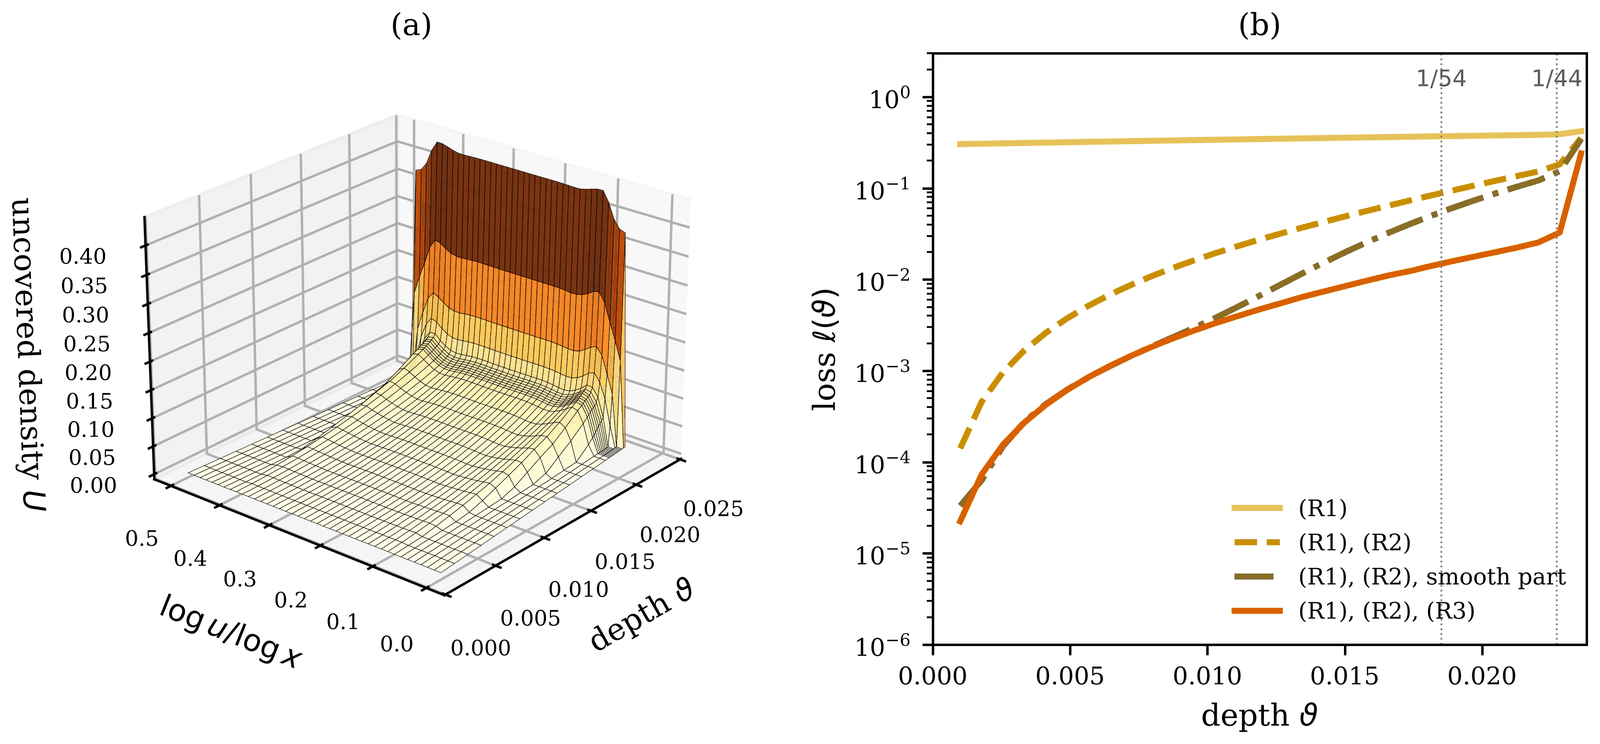
\includegraphics[width=\textwidth]{figures/fig_strips.png}
\caption{(a) The density $U$ of the pairs that fail the rule of Definition~\ref{def:rule}, on the segments $s_1+s_2=\frac12+\vartheta$, as a function of $s_1=\log u/\log x$ and of the depth $\vartheta$. It vanishes where $u$ or $v$ lies in Maynard's window and is largest near $\vartheta=\frac1{42}$. (b) The loss $\ell(\vartheta)$ of \eqref{eq:J} for the rule (R1) alone, for (R1) with (R2), for an intermediate rule that also accepts the part of $uv$ made of primes up to $A$ when it lies in the window, and for the full rule (R1)--(R3). The dotted lines mark $\vartheta=\frac1{54}$ and $\vartheta=\frac1{44}$, where the window changes its shape.}
\label{fig:strips}
\end{figure*}

\section{Remarks}\label{sec:remarks}

\begin{table}[t]
\caption{The constant given by the large sieve for regions of the triangle of Figure~\ref{fig:simplex}. The density is $a=$ (share of the triangle)$\cdot\kappa/4$, and $c=\frac32a^{1/3}$. The rows with strips count them through the rules of Definition~\ref{def:rule}; the row with all of the strips would need a divisor in Maynard's range for every modulus, and the last row would need moduli beyond that range.}
\label{tab:ladder}
\centering
\begin{tabular}{@{}lccc@{}}
\toprule
Region & Share & $a$ & $c$\\
\midrule
One corner & $0.25$ & $0.0284966$ & $0.4582$\\
Two corners & $0.5$ & $0.0569932$ & $0.5773$\\
Three corners & $0.75$ & $0.0854897$ & $0.6608$\\
Strips by (R1) & $0.766883$ & $0.0874142$ & $0.6657$\\
Strips by (R1), (R2) & $0.808696$ & $0.0921802$ & $0.6776$\\
Strips by (R1)--(R3) & $0.814491$ & $0.0928408$ & $0.6792$\\
All of the strips & $0.816327$ & $0.0930501$ & $0.6797$\\
Whole triangle & $1$ & $0.1139863$ & $0.7273$\\
\bottomrule
\end{tabular}
\end{table}

\begin{remark}[Smaller and larger regions]\label{rem:ladder}
The argument applies to any union of corners, and the density is proportional to the area covered (Table~\ref{tab:ladder} and Figure~\ref{fig:ladder}). A single corner gives $c=\frac32(\kappa/16)^{1/3}=0.4582$, two corners give $\frac32(\kappa/8)^{1/3}=0.5773$, and the three corners give $c_0$. Each row with strips includes the three corners; the share of the strips counted by (R1) alone is the closed form $\frac{1181}{1540}$ of Proposition~\ref{prop:var}, and the share of all of the strips is $\frac{40}{49}$.
\end{remark}

\begin{figure}[t]
\centering
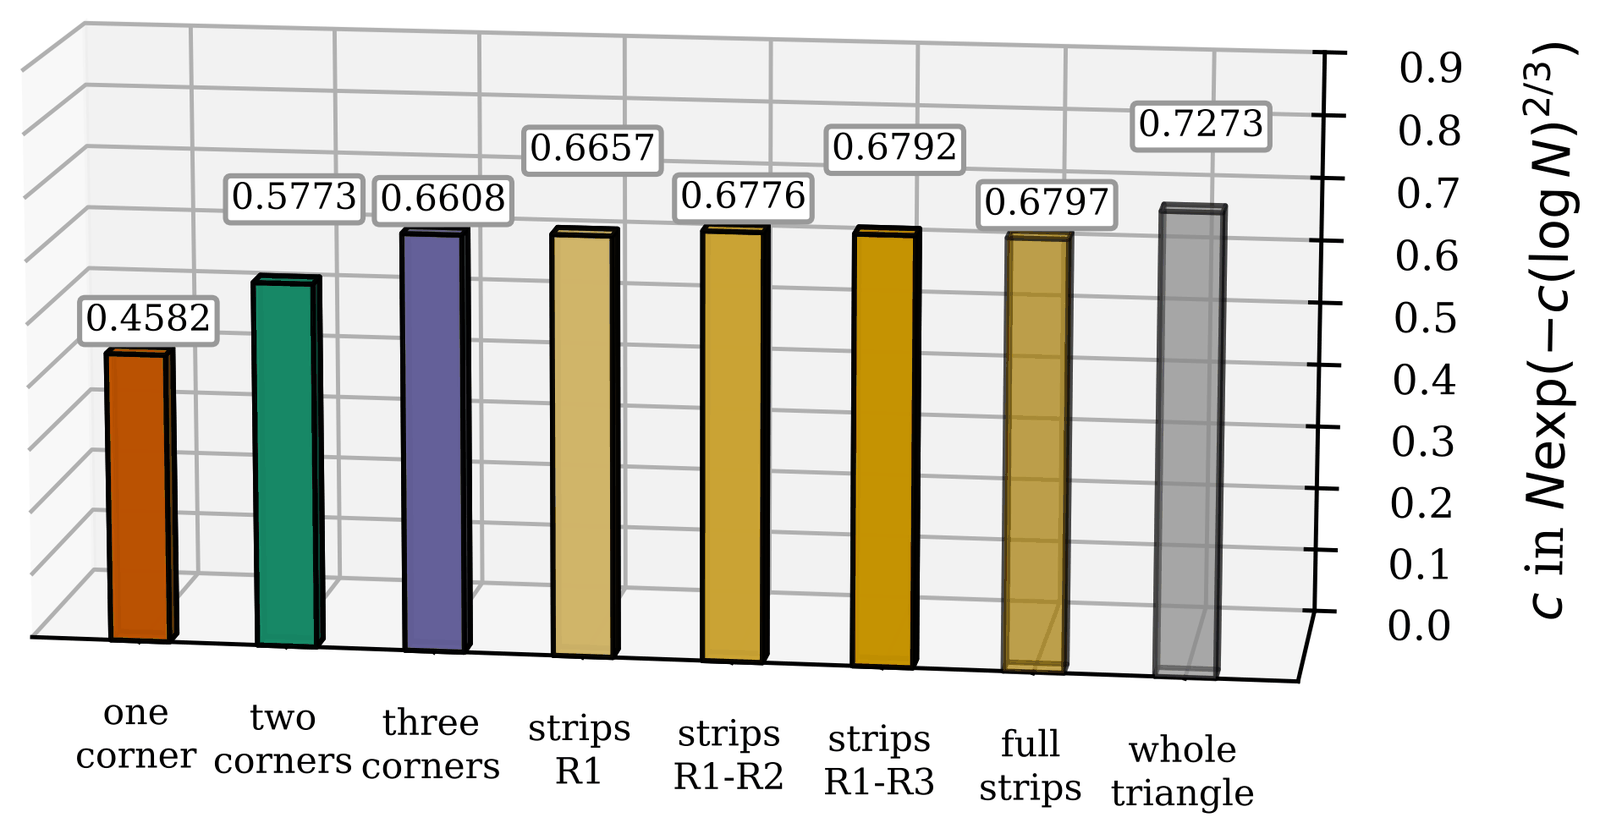
\includegraphics[width=\columnwidth]{figures/fig_ladder.png}
\caption{The constant $c$ in $N\exp(-c(\log N)^{2/3})$ for one, two and three corners, for the corners with the strips counted by the three rules, for the corners with all of the strips, and for the whole triangle, which is not available.}
\label{fig:ladder}
\end{figure}

\begin{remark}[The level]\label{rem:level}
Section~\ref{sec:distinct} uses the level $16X^2\le p$. The factor $16$ does not affect the constants, since only $\log X/\log p\to\frac12$ enters the density, but the bounds \eqref{eq:BC-bounds} do depend on it. For the primes $p\equiv3\pmod4$ below $10^6$ no two triples in the corners at level $\sqrt p/4$ share a class, while at level $\sqrt p/2$ there are $17{,}568$ such pairs, all between $B$ and $C$. The first is at $p=31$, where $(1,4,2)\in B_{31}(2)$ and $(8,1,1)\in C_{31}(2)$ both have the class $8$; here $P=8$, far below the bound $P\ge1024$ of \eqref{eq:BC-bounds}.
\end{remark}

\begin{remark}[Where the method stops]\label{rem:ceiling}
The strips have depth $\frac1{42}$ because the range of divisors in Theorem~\ref{thm:maynard} is empty for $\vartheta\ge\frac1{42}$. If every triple of the strips were counted, the share would be $\frac34+6(\frac1{84}-\frac3{3528})=\frac{40}{49}$ and the constant $\frac32(45/(49\pi^2))^{1/3}=0.6797$; the rule of Definition~\ref{def:rule} loses $6\Jc=0.0018$ of this share. A larger constant needs primes in a fixed residue class to moduli beyond $p^{1/2+1/42}$. Under the Elliott--Halberstam conjecture \cite{EH} the whole centre could be counted through the smallest of the three products, which is at most $P^{2/3}$; since the classes of the centre are distinct and differ from those of the corners apart from the pairs counted by $\nu'(p)$ (Propositions~\ref{prop:centre} and~\ref{prop:centreC}), the whole triangle would then give $\frac32(\kappa/4)^{1/3}=0.7273$.
\end{remark}

\begin{remark}[Vaughan's count of classes]
In the form given in \cite[Section~4]{PW}, Vaughan's argument uses at each prime $f(p)=\lfloor\frac12\sum_{t\mid P}|\mu(t)|\tau(P/t)\rfloor$ classes. The sum equals $\sum_{d\mid P}2^{\omega(d)}$, the number of Type~II triples, so $f(p)$ is half of $|\Tp(p)|$. If the primes are equidistributed in progressions to moduli up to $p^{2/3}$, the number of triples has density $\kappa/4$, the whole triangle, and the classes $f(p)$ have density at most $\kappa/8$. By Proposition~\ref{prop:tilt}(i) and the argument of Theorem~\ref{thm:B}, no sieve with $f(p)$ classes at each prime can then give a constant above $\frac32(\kappa/8)^{1/3}=0.5773$, below both $c_0$ and $c_1$.
\end{remark}

\section{Formal and numerical verification}\label{sec:verification}

The algebraic steps are checked in Lean~4 \cite{Lean} with Mathlib \cite{Mathlib}, in 48 theorems. For the corners: the normal forms \eqref{eq:forms}; the identities \eqref{eq:hj} and \eqref{eq:dj}; the identities \eqref{eq:BC-s}, \eqref{eq:BC-P}, \eqref{eq:BC-M} and \eqref{eq:BC-quad} as consequences of their hypotheses; the three inequalities \eqref{eq:BC-bounds}; the relation $\varphi(qn)=q\,\varphi(n)$ for $q\mid n$; the local factors of $S_B$; the optimisation in Proposition~\ref{prop:tilt}; and the value $c_0^3=729/(256\pi^2)$. For the centre: the Farey bound and the bound $4u^2\alpha<p+1$ of Proposition~\ref{prop:centre}; the identities \eqref{eq:C1}--\eqref{eq:C3}, the inequality $4ks\le a$ and the case $j=0$ of Proposition~\ref{prop:centreC}; and the family of Remark~\ref{rem:family}, with the primality of $531359$ and $1442783$. For the strips: the range of Theorem~\ref{thm:maynard} and the values $\frac1{44}$ and $\frac1{54}$; the divisor chain of Lemma~\ref{lem:chain}; the area $\frac{13}{1176}$ and the share $\frac{40}{49}$. All these theorems depend at most on the axioms \texttt{propext}, \texttt{Classical.choice} and \texttt{Quot.sound}. The analytic estimates of Sections~\ref{sec:counting}, \ref{sec:strips} and~\ref{sec:sieve} are not formalised.

Independent programs in C, C\texttt{++}, Python and Julia check the remaining steps numerically. Over the $332{,}398$ primes $p\equiv3\pmod4$ below $10^7$, with $37{,}093{,}810$ Type~II triples, the corners at level $\sqrt p/16$ are disjoint, the three normal forms agree, the classes in each corner are distinct, and there is no coincidence at all between different corners. The same primes have $6{,}943{,}856$ triples in the centre, of which $1{,}760{,}868$ have their largest coordinate at least $P^{1/2-1/42}$. The classes of the centre are distinct; they agree with no class of $A$ at level $\sqrt p/4$, with no class of $B$ for $u<a$ and no class of $C$ for $u>a$; and the remaining coincidences are the four pairs of Remark~\ref{rem:family}. The divisor chain of Lemma~\ref{lem:chain} holds in all $128{,}000{,}000$ cases of the integers up to $2\cdot10^6$ with 64 windows. The sums $\sum_p|A_p|/p$ and $\sum_p|B_p|/p$ agree with the predictions $\sum_pS_A/p$ and $\sum_pS_B/p$ to within $0.25\%$. The parametrisation of Proposition~\ref{prop:BC} is checked by brute force against all coincidences with $P\le4000$, without the restriction to the corners. The mean values of Lemma~\ref{lem:mean} are computed to $X=2\cdot10^6$, where $(S-\frac\kappa2\log^2X)/\log X$ settles near $-0.47$ for $S_A$ and $0.55$ for $S_B$. The two bounds of Proposition~\ref{prop:tilt} are evaluated for the density $a_0$ up to $T=10^{15}$, where their ratio to the exact optimum is $1.0000$. The integral $\Jc$ is computed as in Section~\ref{sec:constant}.

\emph{The engine runs.} In the first run the library of Anaxia held 22 typed construction nodes: the large sieve with the tilted lower bound; each corner paired with each of the three normal forms, or left out; the centre, left out or counted under the Elliott--Halberstam conjecture; and the inputs that each of these needs. Typed crossing produced 128 closed constructions, which the engine tested on the $39{,}322$ primes $p\equiv3\pmod4$ below $10^6$. It kept 7, those with one, two or three corners and the matching normal forms; it rejected 112 because a normal form failed to separate the classes, 8 that contain the centre because a class of the centre equals a class of a corner at $p=531359$ (Remark~\ref{rem:family}), and the empty construction. The best of the seven gives $c_0$. In the second run the library held 19 nodes for the centre: the three normal forms; five rules for finding a divisor of the modulus in Maynard's range, from (R1) alone to the rule of Definition~\ref{def:rule}, and a rule that omits the bound on the steps of the chain; the family of coincidences of Proposition~\ref{prop:centreC}, allowed or not; and the Elliott--Halberstam conjecture. Of its 37 closed constructions it accepted 5, with the constants $0.660789$ (centre left out), $0.665710$, $0.677596$, $0.678311$ and $0.679210$, marked one as conditional (the whole centre under the Elliott--Halberstam conjecture, $0.727292$), and rejected 31: 24 because the forms $4u^2\alpha$ and $(4a^2\alpha)^{-1}$ do not separate the classes of the centre (they fail on all $12{,}399$ primes tested), 6 because they do not allow the two coincidences of the family below $10^6$, and the rule without the bound on the steps, which claims a divisor that does not exist $1{,}449{,}392$ times among the integers up to $2\cdot10^5$ and 64 windows, first at $n=4$. The best construction is the one of this paper. The records of both runs and the scripts that reproduce them are in the archive \cite{Zen}.

\begin{figure*}[t]
\centering
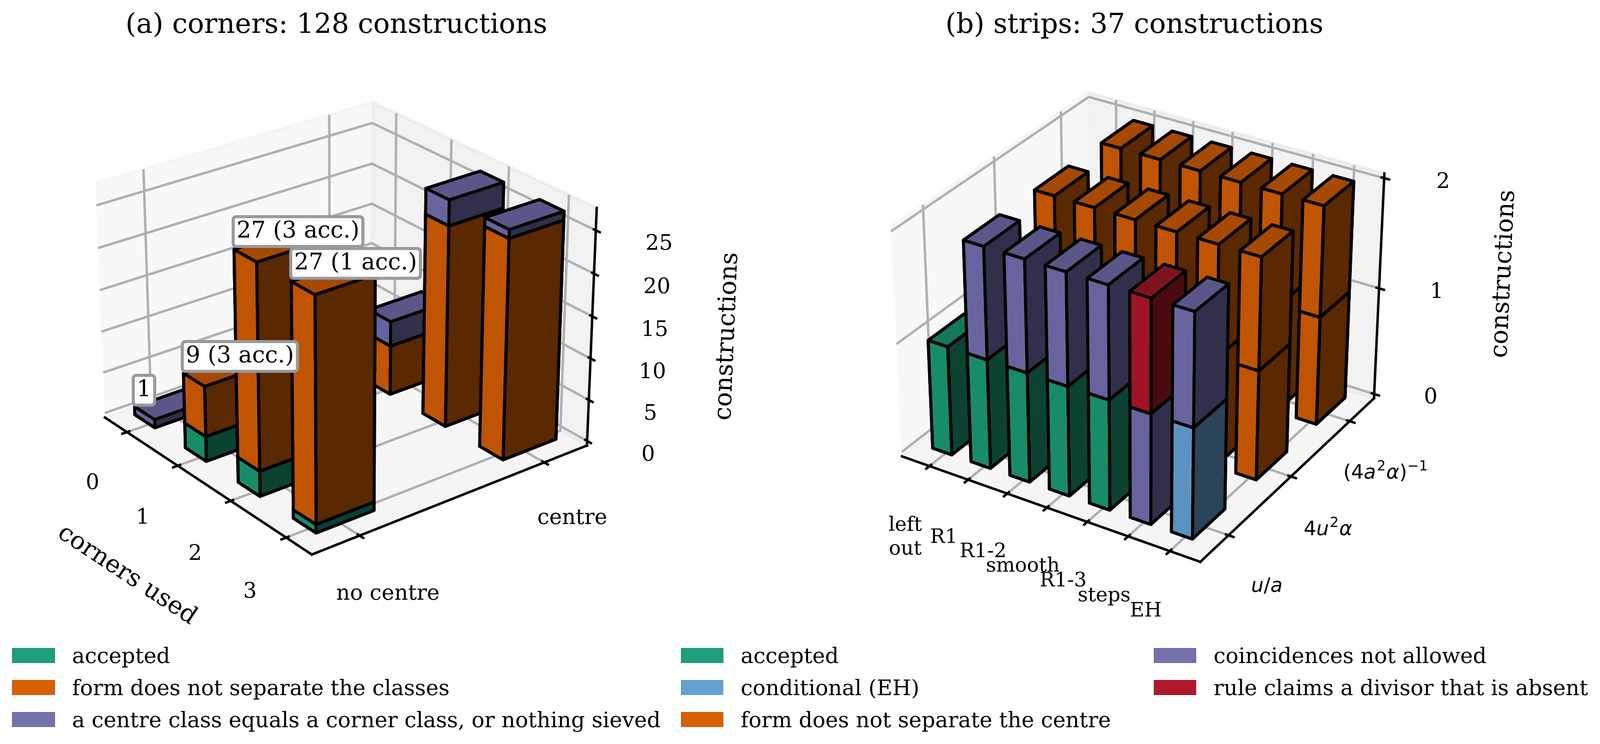
\includegraphics[width=\textwidth]{figures/fig_engine.png}
\caption{The two engine runs. (a) The 128 constructions of the corners, by the number of corners and by whether the centre is included. Seven are accepted; the rest are rejected because a normal form does not separate the classes, because a class of the centre equals a class of a corner, or because they sieve nothing. (b) The 37 constructions of the strips, by the rule that finds the divisor and by the normal form used in the centre, with the family of coincidences allowed (front) or not (back). Five are accepted, and the whole centre under the Elliott--Halberstam conjecture is conditional.}
\label{fig:engine}
\end{figure*}

\appendix

\section{Detailed derivations}\label{app:derivations}

\subsection{The local factors}\label{app:local}

\emph{The totient of $4n$.} If $n$ is odd then $\varphi(4n)=\varphi(4)\varphi(n)=2\varphi(n)$. If $n=2^\beta n'$ with $\beta\ge1$ and $n'$ odd then $\varphi(4n)=2^{\beta+1}\varphi(n')=4\varphi(n)$. In both cases
\begin{equation}\label{eq:phi4n}
\frac1{\varphi(4n)}=\frac{\psi(n)}{2n},\qquad\psi(n)=\prod_{q\mid n,\ q\text{ odd}}\frac q{q-1}.
\end{equation}
For a prime $q$ dividing $n$, $\varphi(qn)=q\,\varphi(n)$.

\emph{The corner $B$.} With \eqref{eq:phi4n},
\[
S_B(X)=\frac12\sum_{u\alpha\le X}\frac{W_B(u,\alpha)}{u\alpha},\qquad W_B(u,\alpha)=\frac{\varphi(u)}u\,\psi(u\alpha).
\]
The function $W_B$ is multiplicative in the pair: $W_B(u,\alpha)=\prod_qW_B(q^{i},q^{j})$ with $q^i\parallel u$ and $q^j\parallel\alpha$. At an odd prime $q$ its local values are $W_B=1$ at $(0,0)$, $W_B=(1-\frac1q)\frac q{q-1}=1$ for $i\ge1$, and $W_B=\frac q{q-1}$ for $i=0$, $j\ge1$. At $q=2$ the factor $\psi$ is absent and $W_B=\frac12$ for $i\ge1$, $W_B=1$ for $i=0$.

The local generating function at an odd prime $q$ is
\[
\sum_{i,j\ge0}W_B(q^i,q^j)x^iy^j=1+\frac x{(1-x)(1-y)}+\frac q{q-1}\cdot\frac y{1-y},
\]
and multiplying by $(1-x)(1-y)$ gives
\[
G_q(x,y)=1+\frac{y}{q-1}-\frac{xy}{q-1}.
\]
At $q=2$ the same computation gives $G_2(x,y)=1-\frac x2$. Hence $W_B(u,\alpha)=\sum_{d\mid u,\,e\mid\alpha}g(d,e)$, where $g$ is multiplicative in the pair with the local values read off from $G_q$: $g(1,q)=\frac1{q-1}$ and $g(q,q)=-\frac1{q-1}$ for odd $q$, $g(2,1)=-\frac12$, and $g=0$ at all other prime powers except $g(1,1)=1$. At $x=y=1/q$,
\[
G_q\Bigl(\frac1q,\frac1q\Bigr)=1+\frac{1}{q(q-1)}-\frac{1}{q^2(q-1)}=1+\frac1{q^2},
\]
and $G_2(\frac12,\frac12)=\frac34$. The same value $1+q^{-2}$ is the quotient of the local sum $\sum_{i,j}W_B(q^i,q^j)q^{-i-j}=(q^2+1)/(q-1)^2$ by $(1-1/q)^{-2}$.

\emph{The corner $A$.} Here
\[
S_A(X)+R(X)=\frac12\sum_{ua\le X}\frac{W_A(u,a)}{ua},
\]
where $W_A(u,a)=\psi(ua)$ when $\gcd(u,a)=1$, $W_A=0$ otherwise, and $R(X)$ is the sum over the pairs with $u=1$ or $a=1$. Since $\sum_{n\le X}1/\varphi(4n)=O(\log X)$, $R(X)=O(\log X)$. The local values of $W_A$ at an odd prime are $1$ at $(0,0)$, $\frac q{q-1}$ when exactly one exponent is positive, and $0$ when both are; at $q=2$ they are $1,1,0$. The local generating functions after multiplication by $(1-x)(1-y)$ are
\[
G^A_q(x,y)=1+\frac{x+y}{q-1}-\frac{(q+1)xy}{q-1},\qquad G^A_2=1-xy,
\]
with $G^A_q(\frac1q,\frac1q)=1+q^{-2}$ and $G^A_2(\frac12,\frac12)=\frac34$. The coefficients give $W_A=\sum_{d\mid u,\,e\mid a}h_A(d,e)$ with $\sum_{d,e}|h_A(d,e)|/(de)<\infty$, as Lemma~\ref{lem:density} requires, and the same holds for $g$.

\begin{table}[h]
\caption{The local factors of the two mean values. Both corners give $1+q^{-2}$ at odd $q$ and $\frac34$ at $2$.}
\label{tab:local}
\centering
\begin{tabular}{@{}lccc@{}}
\toprule
& $G(x,y)$ at odd $q$ & at $x=y=\frac1q$ & $q=2$\\
\midrule
$B$ & $1+\frac{y-xy}{q-1}$ & $1+q^{-2}$ & $\frac34$\\
$A$ & $1+\frac{x+y-(q+1)xy}{q-1}$ & $1+q^{-2}$ & $\frac34$\\
\bottomrule
\end{tabular}
\end{table}

\emph{The constant.} The Euler product of the values at $x=y=1/q$ is
\[
\frac34\prod_{q\ \mathrm{odd}}\Bigl(1+\frac1{q^2}\Bigr)=\frac34\cdot\frac45\cdot\frac{\zeta(2)}{\zeta(4)}=\frac34\cdot\frac45\cdot\frac{15}{\pi^2}=\frac9{\pi^2}=2\kappa,
\]
using $\zeta(2)=\pi^2/6$ and $\zeta(4)=\pi^4/90$.

\subsection{The hyperbola sum}\label{app:hyperbola}

For $Y\ge1$ let $H(Y)=\sum_{mn\le Y}1/(mn)$ and $H(Y)=0$ for $Y<1$. With $h(x)=\sum_{m\le x}1/m=\log x+\gamma+O(1/x)$,
\[
H(Y)=\sum_{m\le Y}\frac1m\,h\Bigl(\frac Ym\Bigr)=\sum_{m\le Y}\frac{\log Y-\log m+\gamma}m+O\Bigl(\frac{\log Y}Y\Bigr).
\]
Since $\sum_{m\le Y}(\log m)/m=\frac12\log^2Y+O(1)$, this gives $H(Y)=\frac12\log^2Y+2\gamma\log Y+O(1)$.

Write $\Lambda=\log X$. Then, with $g$ as in Appendix~\ref{app:local},
\[
2S_B(X)=\sum_{de\le X}\frac{g(d,e)}{de}\Bigl(\frac12(\Lambda-\log de)^2+O(1+\Lambda)\Bigr).
\]
The series $\sum_{d,e}|g(d,e)|(1+\log de)^2/(de)$ converges, since its Euler factor at an odd $q$ is $1+O(q^{-2}\log^2q)$. For the pairs with $de>X$, $\sum_{de>X}|g(d,e)|/(de)\le X^{-1/4}\sum_{d,e}|g(d,e)|(de)^{-3/4}$, and the last series converges because its terms at $q$ are $O(q^{-7/4})$ and $O(q^{-5/2})$. Expanding the square,
\[
2S_B(X)=\frac{\Lambda^2}2\sum_{d,e}\frac{g(d,e)}{de}+O(\Lambda)=\kappa\Lambda^2+O(\Lambda).
\]
For $S_A$ the coefficients of $G^A_q$ are of size $q^{-1}$ at $(1,0)$ and $(0,1)$ and of size $1$ at $(1,1)$, so the terms of $\sum|h_A(d,e)|(de)^{-3/4}$ at $q$ are $O(q^{-7/4})$ and $O(q^{-3/2})$; the rest is identical.

\subsection{The Bombieri--Vinogradov theorem with multiplicities}\label{app:bv}

The Bombieri--Vinogradov theorem \cite{Bom}, \cite[Chapter~28]{Dav} states that for every $A>0$ there is $B>0$ such that
\[
\sum_{q\le x^{1/2}(\log x)^{-B}}\max_{(b,q)=1}\max_{y\le x}\Bigl|\pi(y;q,b)-\frac{\pi(y)}{\varphi(q)}\Bigr|\ll_A\frac x{(\log x)^A}.
\]
Let $E(q)$ be the inner maximum. In the proof of Proposition~\ref{prop:primes} each modulus $q=4n$ occurs with multiplicity at most $\tau_3(n)$. Using the trivial bound $E(q)\ll x/q$, Cauchy's inequality and $\sum_{n\le x}\tau_3(n)^2/n\ll(\log x)^9$,
\begin{align*}
\sum_q\tau_3(q)E(q)&\le\Bigl(\sum_q\tau_3(q)^2E(q)\Bigr)^{1/2}\Bigl(\sum_qE(q)\Bigr)^{1/2}\\
&\ll\frac{x}{(\log x)^{(A-9)/2}}.
\end{align*}
Taking $A=15$ gives the error $O(x(\log x)^{-3})$ used in the proof. The inclusion--exclusion over $d\mid(u,P_z)$ replaces each pair by the progressions modulo $4u\alpha d$ with $d\mid u$; a modulus $4m$ arises from at most $\tau_3(m)$ triples $(u,\alpha,d)$, so the same estimate covers all of them. The moduli $4u\alpha d\le4X_je^{2z}$, since $\prod_{q\le z}q\le e^{2z}$, are below $x^{1/2}(\log x)^{-B}$ for $j$ large because $X_j=2^{j(1/2-\delta)}$ and $z=j^{1/2}$.

\subsection{Maynard's theorem with multiplicities}\label{app:maynard}

In the proof of Proposition~\ref{prop:strips}, fix $y\in[x,2x]$ and let $E(q;y)=|\pi(y;q,-1)-\pi(y)/\varphi(q)|$. For $q\le y$ we have $E(q;y)\le\pi(y;q,-1)+\pi(y)/\varphi(q)\ll y\log\log y/q$, and each modulus $q$ that occurs lies in $Q_{\vartheta_i^+,\eta}(y)$ and occurs at most $\tau_3(q/4)$ times. Since $\sum_{n\le y}\tau_3(n)^2/n\ll(\log y)^9$, the sum of $\tau_3(q/4)^2E(q;y)$ over these moduli is $O(y(\log y)^{10})$, and by Theorem~\ref{thm:maynard} with $A=17$ the sum of $E(q;y)$ is $O(y(\log y)^{-17})$. Cauchy's inequality gives
\[
\sum_q\tau_3(q/4)\,E(q;y)\ll\frac y{(\log y)^{7/2}}.
\]
Let $f(p)=|\Zc^A_{p,i}|$ and $F(y)=\sum_{x<p\le y}f(p)$, and let $S$ be the sum of $1/\varphi(4ua)$ over the pairs $(u,a)$ of the proof of Proposition~\ref{prop:strips}. Applying the bound at $y$ and at $x$ gives $F(y)=(\pi(y)-\pi(x))S+O(x(\log x)^{-7/2})$ at each of the $j+1$ points $y_l=x(1+l/j)$. On $(y_l,y_{l+1}]$ the weight $1/p$ lies between $1/y_{l+1}$ and $1/y_l$, whose ratio is at most $1+1/j$, and $f\ge0$, so
\[
\sum_{y_l<p\le y_{l+1}}\frac{f(p)}p=\frac{F(y_{l+1})-F(y_l)}{y_l}\Bigl(1+O\Bigl(\frac1j\Bigr)\Bigr).
\]
The same holds with $f$ replaced by $S$ times the indicator of the primes. Summing over $l$,
\[
\sum_{p\in I_j}\frac{f(p)}p=S\sum_{p\in I_j}\frac1p\Bigl(1+O\Bigl(\frac1j\Bigr)\Bigr)+O\bigl(j(\log x)^{-7/2}\bigr).
\]
Since $S\ll j^2$ and $\sum_{p\in I_j}1/p\ll1/j$, the error is $O(1)$. The piece $B$ is treated in the same way with the moduli $4u\alpha d$.

\subsection{Large prime factors of \texorpdfstring{$\gcd(u,a)$}{gcd(u,a)}}\label{app:large}

\emph{The truncated product.} For $u\ge1$,
\[
0\le\prod_{\substack{q\mid u\\ q\le z}}\Bigl(1-\frac1q\Bigr)-\frac{\varphi(u)}u\le\sum_{\substack{q\mid u\\ q>z}}\frac1q.
\]
Writing $u=qu'$ and using $\varphi(4qu'\alpha)\ge(q-1)\varphi(4u'\alpha)$,
\[
S_B^{(z)}(X)-S_B(X)\le\sum_{q>z}\frac1{q(q-1)}\sum_{u'\alpha\le X}\frac1{\varphi(4u'\alpha)}\ll\frac{\log^2X}z,
\]
because $\sum_{n\le X}\tau(n)/\varphi(4n)\ll\log^2X$. The same bound, with $X=x^K$, controls the difference of the weights in the piece $B$ of Proposition~\ref{prop:strips}.

\emph{The pairs with a common prime $q>z$.} Such a pair satisfies $p\equiv-1\pmod{4u\alpha q}$ with $q\mid u$, and $m=4u\alpha q\le4X_j^2\le4\cdot2^{j(1-2\delta)}$. For $x=2^{j+1}$ we have $\log(x/m)\ge\delta j\log2$ when $j\ge3/\delta$. The Brun--Titchmarsh inequality $\pi(x;m,b)\le2x/(\varphi(m)\log(x/m))$ \cite{MV} gives
\[
\pi(x;m,-1)\le\frac{2\cdot2^{j+1}}{\varphi(m)\,\delta j\log2}\le\frac{5\,\pi(I_j)}{\delta\,\varphi(m)}
\]
for $j$ large, since $\pi(I_j)\sim2^j/(j\log2)$. Summing over $q>z$ and the pairs, with $\varphi(4u\alpha q)=q\,\varphi(4u\alpha)$, the total over $p\in I_j$ is at most
\[
\frac{5\,\pi(I_j)}\delta\sum_{q>z}\frac1{q(q-1)}\sum_{u'\alpha\le X_j}\frac1{\varphi(4u'\alpha)}\ll\frac{\pi(I_j)\log^2X_j}{\delta z}.
\]
With the weight $1/p\le2^{-j}$ this contributes $O(j/(\delta z))$ to $\sum_{p\in I_j}|B_p|/p$.

\subsection{Large common prime factors in the strips}\label{app:Blarge}

In the piece $B$ of Proposition~\ref{prop:strips} the pairs $(u,\alpha)$ satisfy $u\alpha\le x^{1/2+1/42}$. A pair whose $u$ and $a$ share a prime $q>z$ satisfies $p\equiv-1\pmod m$ with $m=4u\alpha q$, $q\mid u$. If $q\le x^{1/3}$, then $m\le4x^{1/2+1/42+1/3}$, so $\log(2x/m)\ge\frac18\log x$, and the Brun--Titchmarsh inequality gives $\pi(2x;m,-1)\ll x/(\varphi(m)\log x)$. As in Appendix~\ref{app:large}, the sum over $q>z$ and the pairs is $\ll(x/\log x)(\log x)^2/z$, and with the weight $1/p\le1/x$ it contributes $O(j/z)$. If $q>x^{1/3}$, we use $\pi(2x;m,-1)\le2x/m+1$. Writing $u=qu'$, the first term gives
\[
\sum_{q>x^{1/3}}\frac{2x}{4q^2}\sum_{u'\alpha\le x}\frac1{u'\alpha}\ll x^{2/3}(\log x)^2,
\]
and the second term is at most the number of triples $(q,u',\alpha)$ with $qu'\alpha\le x^{1/2+1/42}$, which is $O(x^{0.53})$. With the weight $1/p\le1/x$ both are $o(1)$.

\subsection{The density of the pairs that fail}\label{app:density}

\emph{Profiles.} Fix $\xi>0$. For $x>1$ and $n\ge1$, the $\xi$-profile of $n$ is the pair $\Pi_x(n)=(t,Z)$, where $t=\log T(n)/\log x$, with $T(n)$ the product of the prime powers of $n$ whose prime is below $x^\xi$, and $Z$ is the multiset of the numbers $\log q/\log x$ over the prime factors $q\ge x^\xi$ of $n$, counted with multiplicity. The size of $n$ is $s=t+\sum Z$. On the space of profiles let
\[
\lambda_1=\rho(t/\xi)\,dt\otimes\nu,\qquad\nu=\delta_\varnothing+\sum_{k\ge1}\frac1{k!}\prod_{i=1}^k\frac{\one[z_i\ge\xi]\,dz_i}{z_i},
\]
where $\nu$ is a measure on finite multisets $\{z_1,\dots,z_k\}$. Every $n$ factors uniquely as $n=T(n)\,r$ with $r$ free of primes below $x^\xi$, and $1/n=(1/T(n))(1/r)$. By the theorem of Dickman and de Bruijn \cite[Chapter~III.5]{Ten}, $\Psi(X,X^{1/v})=X\rho(v)(1+o(1))$ uniformly for bounded $v$, and partial summation gives
\[
\sum_{\substack{T\le x^t\\T\ x^\xi\text{-smooth}}}\frac1T=\log x\int_0^t\rho\Bigl(\frac\tau\xi\Bigr)d\tau+o(\log x)
\]
uniformly for bounded $t$. By Mertens' theorem,
\[
\sum_{x^z<q\le x^{z'}}\frac1q=\log\frac{z'}z+o(1)\qquad(\xi\le z<z'),
\]
and the numbers $r$ with a repeated prime factor $q\ge x^\xi$ have total weight $O(x^{-\xi})$ relative to the others. Hence, for every bounded set $F$ of profiles whose boundary is $\lambda_1$-null,
\[
\frac1{\log x}\sum_{n:\ \Pi_x(n)\in F}\frac1n\to\lambda_1(F).
\]
Since the weight $1/(uv)$ is a product, the same holds for pairs: $(\log x)^{-2}\sum_{(\Pi_x(u),\Pi_x(v))\in F}1/(uv)\to\lambda_1\otimes\lambda_1(F)$ for every bounded $F$ with $\lambda_1\otimes\lambda_1$-null boundary. The image of $\lambda_1$ under the size $s$ is Lebesgue measure, since $\sum_{n\le x^s}1/n=s\log x+O(1)$.

\emph{The failure set.} Let $\xi=\min(\theta^+-\theta^-,\theta^-)$, so that $G=x^\xi$ for the window $(x^{\theta^-},x^{\theta^+})$. The pair $(u,v)$ fails the rule exactly when its profiles $(t_1,Z_1)$, $(t_2,Z_2)$ satisfy: $s_1,s_2\notin(\theta^-,\theta^+)$; no element of $Z_1\cup Z_2$ lies in $(\theta^-,\theta^+)$; and the largest element of $(Z_1\cup Z_2)\cap[\xi,\theta^-]$, or $0$ if there is none, plus $t_1+t_2$ is at most $\theta^-$. When $s_1,s_2>\theta^-$, the last two conditions say that $t_1+t_2\le\theta^-$ and that every element of $Z_1\cup Z_2$ lies in $\mathcal A_w$ with $w=\max(\theta^--t_1-t_2,\xi)$, up to the $\lambda_1$-null event that an element equals $\xi$. The boundary of the failure set lies in the union of the sets where $s_i$, an element of $Z_1\cup Z_2$, or the sum in the last condition takes one of the values $\xi$, $\theta^-$, $\theta^+$, which are $\lambda_1\otimes\lambda_1$-null on $\{s_1,s_2>\theta^-\}$. For fixed $t_i$, the density of $\sum Z_i$ over the multisets in $\mathcal A_w$ is $\varpi_w$: writing $f$ for this density, $r f(r)$ is the $\nu$-integral of $\sum_iz_i$ over the multisets with sum $r$, and by the symmetry of $\nu$ this equals $\one_{\mathcal A_w}(r)+\int_{\mathcal A_w\cap(0,r)}f(r-z)\,dz$, which is \eqref{eq:varpi}. The empty multiset would give $s_i=t_i\le\theta^-$, which is excluded. Hence the $\lambda_1\otimes\lambda_1$-measure of the failing profiles with $(s_1,s_2)\in R$ is $\iint_RU$.

\emph{The bound $0\le U\le1$.} Let $\varpi$ be the solution of \eqref{eq:varpi} with $\mathcal A_w$ replaced by $(\xi,\infty)$, the density of $\sum Z$ over all multisets. Then $0\le\varpi_w\le\varpi$, and dropping the condition $t_1+t_2\le\theta^-$ in \eqref{eq:U},
\[
U(s_1,s_2)\le\prod_{i=1}^2\int_0^{s_i}\rho\Bigl(\frac{t}{\xi}\Bigr)\varpi(s_i-t)\,dt\le1,
\]
because each factor is the $\lambda_1$-density at $s_i$ of the profiles with a nonempty multiset, and the total density is $1$.

\emph{Proof of Lemma~\ref{lem:density}.} For $h=\one_{(1,1)}$ the statement is the convergence above, applied to the passing profiles with $(s_1,s_2)\in R$, which form a bounded set with null boundary and have measure $\iint_R(1-U)$. For general $h$,
\[
\sum_{(u,v)}\frac{W(u,v)}{uv}=\sum_{d,e}\frac{h(d,e)}{de}\sum_{(u',v')}\frac1{u'v'},
\]
where $(u',v')$ runs over the pairs for which $(du',ev')$ passes and has its sizes in $R$. For fixed $d,e$ and $x^\xi$ larger than every prime factor of $de$, the profiles of $du'$ and $ev'$ are those of $u'$ and $v'$ with $t$ increased by $\log d/\log x$ and $\log e/\log x$, which tend to $0$; since the limit set has null boundary, the inner sum is $(\log x)^2\iint_R(1-U)+o((\log x)^2)$. It is also at most $\sum_{u',v'\le x^K}1/(u'v')\ll(\log x)^2$, so dominated convergence over $(d,e)$ with $\sum|h(d,e)|/(de)<\infty$ gives the lemma.

\emph{Proof of the limit in Lemma~\ref{lem:limit}.} Fix $\eta_0>0$. For $\vartheta\in[\eta_0,\frac1{42}-\eta_0]$ the number $\xi(\vartheta)=\min(\theta(\vartheta)-2\vartheta,2\vartheta)$ is at least $\xi_0=\min(\frac2{105},2\eta_0)$, and the same holds for the windows $(\theta_i^-,\theta_i^+)$ with $\vartheta_i\in[\eta_0,\frac1{42}-\eta_0]$ once $\delta$ is small. The $\xi$-profile of a number is a function of its $\xi_0$-profile, so all these failure sets live in the space of $\xi_0$-profiles with the measure $\lambda_1\otimes\lambda_1$ at level $\xi_0$, and $\sum_i\iint_{R_i}U_i$, restricted to these depths, is the measure of the set of profile pairs with $\vartheta=s_1+s_2-\frac12$ in the range and $(s_1,s_2)$ in $\bigcup_iR_i$ that fail the rule for the window of their piece. As $\delta\to0$ these windows converge to $(2\vartheta,\theta(\vartheta))$, and outside a null set of profiles the indicator of failure converges to that for the limiting window. The sets lie in a fixed bounded region of finite measure, so by dominated convergence the measure tends to $\int_{\eta_0}^{1/42-\eta_0}\ell(\vartheta)\,d\vartheta$. The depths outside $[\eta_0,\frac1{42}-\eta_0]$ contribute $O(\eta_0)$ to both sides, because $0\le U\le1$, and $\eta_0$ is arbitrary.

\subsection{Partial summation in a block}\label{app:block}

Let $f(p)\ge0$ and $F(y)=\sum_{2^j<p\le y}f(p)$ for $y\in I_j$. Suppose $F(y)=(\pi(y)-\pi(2^j))S+E(y)$ with $|E(y)|\le E$ for all $y\in I_j$. Then
\begin{align*}
\sum_{p\in I_j}\frac{f(p)}p&=\frac{F(2^{j+1})}{2^{j+1}}+\int_{2^j}^{2^{j+1}}\frac{F(y)}{y^2}\,dy\\
&=S\sum_{p\in I_j}\frac1p+O\Bigl(\frac E{2^j}\Bigr),
\end{align*}
because the same identity holds for $\pi(y)-\pi(2^j)$ in place of $F$ and $\int_{2^j}^{2^{j+1}}y^{-2}\,dy=2^{-j-1}$. With $E\ll2^j(\log2^j)^{-3}$ the error is $O(j^{-3})$. The pairs removed in Appendix~\ref{app:large} are handled with the trivial weight $1/p\le2^{-j}$. Finally, the prime number theorem with the error term $O(y\exp(-c\sqrt{\log y}))$ gives $\sum_{p\le y}1/p=\log\log y+M_1+O(\exp(-c\sqrt{\log y}))$, so $\sum_{p\in I_j}1/p=\log(1+1/j)+O(e^{-c\sqrt j})=1/j+O(1/j^2)$.

\subsection{From the density to the Euler product}\label{app:abel}

Let $N(\lambda)=\sum_{p\le e^\lambda}\omega(p)/p$ and $G_0(\sigma)=\sum_p(\omega(p)/p)p^{-\sigma}$. Since $N(\lambda)=O(\lambda^2)$, integration by parts gives
\[
G_0(\sigma)=\int_0^\infty e^{-\sigma\lambda}\,dN(\lambda)=\sigma\int_0^\infty e^{-\sigma\lambda}N(\lambda)\,d\lambda.
\]
If $N(\lambda)\le(a+\eps)\lambda^2+C_\eps$, then $G_0(\sigma)\le(a+\eps)\sigma\cdot2\sigma^{-3}+C_\eps=2(a+\eps)\sigma^{-2}+C_\eps$. In the same way
\begin{align*}
\sum_p\frac{\omega(p)\log p}{p^{1+\sigma}}&=\int_0^\infty N(\lambda)(\sigma\lambda-1)e^{-\sigma\lambda}\,d\lambda,\\
\sum_p\frac{\omega(p)\log^2p}{p^{1+\sigma}}&=\int_0^\infty N(\lambda)(\sigma\lambda^2-2\lambda)e^{-\sigma\lambda}\,d\lambda,
\end{align*}
and, when $N(\lambda)=(a+o(1))\lambda^2$, these are $(4a+o(1))\sigma^{-3}$ and $(12a+o(1))\sigma^{-4}$ as $\sigma\to0^+$, from $\int_0^\infty\lambda^2(\sigma\lambda-1)e^{-\sigma\lambda}d\lambda=4\sigma^{-3}$ and $\int_0^\infty\lambda^2(\sigma\lambda^2-2\lambda)e^{-\sigma\lambda}d\lambda=12\sigma^{-4}$. If the sums are restricted to $p\le Q=e^T$, the same asymptotics hold provided $\sigma T\to\infty$, since the tails are bounded by $\sigma^{-k}\int_{\sigma T}^\infty x^{k+1}e^{-x}\,dx$ with $k=2,3,4$. Finally $0\le g(p)-\omega(p)/p\le2\omega(p)^2/p^2$ once $\omega(p)\le p/2$, which holds for all large $p$ because $\omega(p)\le C_\eta p^\eta$; hence $F(\sigma)=G_0(\sigma)+O(1)$, and the same holds for the sums with $\log p$ and $\log^2p$.

\subsection{The choice of \texorpdfstring{$\sigma$}{sigma}}\label{app:sigma}

Assume $N(\lambda)=(a+o(1))\lambda^2$ with $a>0$. With $y_p=g(p)p^{-\sigma}$ and $\pi_p=y_p/(1+y_p)$,
\[
\mu_\sigma=\sum_{p\le Q}\pi_p\log p,\qquad V_\sigma=\sum_{p\le Q}\pi_p(1-\pi_p)\log^2p.
\]
Both are continuous in $\sigma$, and both tend to $0$ as $\sigma\to\infty$ because the sums are finite. Since $y_p-y_p^2\le\pi_p\le y_p$, Appendix~\ref{app:abel} gives, whenever $\sigma T\to\infty$,
\[
\mu_\sigma=(4a+o(1))\sigma^{-3},\qquad V_\sigma\le(12a+o(1))\sigma^{-4}.
\]
Take $\sigma_1=\eps_0T^{-1/3}$ with $\eps_0>0$ small. Then $\sigma_1T\to\infty$ and $\mu_{\sigma_1}\ge3a\eps_0^{-3}T>T$, so by continuity there is $\sigma\ge\sigma_1$ with $\mu_\sigma+\sqrt{2V_\sigma}=T$. If $\sigma T$ stayed bounded along a sequence of $T$, say $\sigma T\le K$, then $p^{-\sigma}\ge e^{-K}$ for $p\le Q$ and
\[
\mu_\sigma\ge\frac{e^{-K}}2\sum_{p\le Q}\frac{\omega(p)\log p}p\gg e^{-K}T^3,
\]
contradicting $\mu_\sigma\le T$ for large $T$. Hence $\sigma T\to\infty$, the asymptotics apply, and $\mu_\sigma\le T$ gives $\sigma\ge(4a-o(1))^{1/3}T^{-1/3}$, while $\sigma\ge\sigma_1$ already gives $\sigma\gg T^{-1/3}$ from below and $T=\mu_\sigma+\sqrt{2V_\sigma}\ll\sigma^{-3}$ gives $\sigma\ll T^{-1/3}$. Therefore $\sigma\sqrt{2V_\sigma}\ll\sigma^{-1}\ll T^{1/3}$. Finally
\[
\sum_{p\le Q}\log(1+y_p)\ge\sum_{p\le Q}y_p-\frac12\sum_py_p^2\ge F_Q(\sigma)-O(1),
\]
where $F_Q$ is $F$ restricted to $p\le Q$, and $F_Q(\sigma)=(2a+o(1))\sigma^{-2}$ by Appendix~\ref{app:abel}. This is what the proof of Proposition~\ref{prop:tilt}(ii) uses.

\subsection{The band below \texorpdfstring{$\sqrt p$}{sqrt p}}\label{app:band}

Proposition~\ref{prop:upper} uses the following count. For $p\in I_j$ take the pairs $(u,\alpha)$ with $p^{1/2-\delta}<u\alpha\le p^{1/2}$ and $p\equiv-1\pmod{4u\alpha}$; the corners $A$ and $C$ are treated in the same way. Every such pair has $2^{j(1/2-\delta)}<u\alpha\le2^{(j+1)/2}$, and the modulus $m=4u\alpha$ satisfies $\log(2^{j+1}/m)\ge(\frac j2-2)\log2$. The Brun--Titchmarsh inequality gives $\pi(2^{j+1};m,-1)\le(9+o(1))\pi(I_j)/\varphi(m)$, so the number of these pairs, summed over $p\in I_j$, is at most
\[
(9+o(1))\,\pi(I_j)\sum_{2^{j(1/2-\delta)}<n\le2^{(j+1)/2}}\frac{\tau(n)}{\varphi(4n)}.
\]
The sum over $n$ is $O(\log^2(2^{j/2})-\log^2(2^{j(1/2-\delta)}))+O(j)=O(\delta j^2)+O(j)$. With the weight $1/p\le2^{-j}$, the contribution of the block is $O(\delta j)+O(1)$, and the sum over $j\le J$ is $O(\delta J^2)+O(J)=O(\delta\lambda^2)+O(\lambda)$.

\section*{Data availability}
\begingroup\raggedright
The \LaTeX{} source of this paper, the Lean~4 formalisation and the C, C\texttt{++}, Python, Julia and shell programs described in Section~\ref{sec:verification}, the records of the two engine runs and the scripts that reproduce them are available at \url{\repoURL} and in the archive \cite{Zen}. The corners, the treatment of the centre and the rule of Definition~\ref{def:rule} were selected with the engine Anaxia of the BLLM project \cite{Ana,BLLM}, version 3.0.5, in the two runs described in Section~\ref{sec:verification}. Deep Bhattacharjee carried out the computations and the Lean, C, C\texttt{++}, Python, Julia and shell verifications, and the proofs and the text were drafted, with AI assistance (Claude, Anthropic); both authors approved the final version.\par
\endgroup

\section*{Funding}
None.

\section*{Competing interests}
None.

\makeatletter
\def\bibsection{\par\begingroup\baselineskip26\p@\bib@device{\hsize}{72\p@}\endgroup\nobreak\@nobreaktrue\addvspace{19\p@}}
\makeatother
\begingroup\raggedright
\begin{thebibliography}{99}

\bibitem{Ana}
D.~Bhattacharjee, \emph{BLLM: Beyond the LLM with Deep Human-Mind-AI}, software archive with the engine Anaxia, version 3.0.5, Zenodo, 2026, doi:\href{https://doi.org/10.5281/zenodo.23469389}{10.5281/zenodo.23469389}; all versions: doi:\href{https://doi.org/10.5281/zenodo.23286641}{10.5281/zenodo.23286641}.

\bibitem{BLLM}
D.~Bhattacharjee and U.~Bhattacharya, \emph{BLLM: Beyond the LLM with Deep Human-Mind-AI}, 2026, paper in the archive \cite{Ana}.

\bibitem{BB26}
D.~Bhattacharjee and U.~Bhattacharya, \emph{Maximal large sieve and coefficient uniform failure for Liouville correlations}, Preprints.org, 2026, doi:\href{https://doi.org/10.20944/preprints202606.1350.v1}{10.20944/preprints202606.1350.v1}.

\bibitem{BBv1}
D.~Bhattacharjee and U.~Bhattacharya, \emph{A power-saving asymptotic for the two-parameter Type~II sieve sum of the Erd\H{o}s--Straus equation}, 2026, paper in the archive \cite{Zen}.

\bibitem{Bom}
E.~Bombieri, \emph{On the large sieve}, Mathematika \textbf{12} (1965), 201--225, doi:\href{https://doi.org/10.1112/S0025579300005313}{10.1112/S0025579300005313}.

\bibitem{Dah}
B.~Dahan, \emph{Sieve dimension and search depth for the Erd\H{o}s--Straus conjecture, $n\equiv1\pmod{24}$}, arXiv:\href{https://arxiv.org/abs/2608.24035}{2608.24035}, 2026.

\bibitem{Dav}
H.~Davenport, \emph{Multiplicative Number Theory}, 2nd ed., Graduate Texts in Mathematics 74, Springer, New York, 1980, doi:\href{https://doi.org/10.1007/978-1-4757-5927-3}{10.1007/978-1-4757-5927-3}.

\bibitem{Dya}
E.~Dyachenko, \emph{Constructive proofs of the Erd\H{o}s--Straus conjecture for prime numbers with $P$ congruent to $1$ modulo $4$}, arXiv:\href{https://arxiv.org/abs/2511.07465}{2511.07465}, 2025.

\bibitem{EH}
P.~D.~T.~A.~Elliott and H.~Halberstam, \emph{A conjecture in prime number theory}, in: Symposia Mathematica, Vol.~IV (INDAM, Rome, 1968/69), Academic Press, London, 1970, pp.~59--72.

\bibitem{ET}
C.~Elsholtz and T.~Tao, \emph{Counting the number of solutions to the Erd\H{o}s--Straus equation on unit fractions}, J. Aust. Math. Soc. \textbf{94} (2013), 50--105, doi:\href{https://doi.org/10.1017/S1446788712000468}{10.1017/S1446788712000468}.

\bibitem{Guy}
R.~K.~Guy, \emph{Unsolved Problems in Number Theory}, 3rd ed., Problem Books in Mathematics, Springer, New York, 2004, doi:\href{https://doi.org/10.1007/978-0-387-26677-0}{10.1007/978-0-387-26677-0}.

\bibitem{Lean}
L.~de~Moura and S.~Ullrich, \emph{The Lean~4 theorem prover and programming language}, in: Automated Deduction -- CADE 28, Lecture Notes in Comput. Sci. 12699, Springer, 2021, pp.~625--635, doi:\href{https://doi.org/10.1007/978-3-030-79876-5_37}{10.1007/978-3-030-79876-5\_37}.

\bibitem{Liu}
Z.~Liu, \emph{The exact reciprocal-totient constant in the two-parameter Erd\H{o}s--Straus sieve}, preprint, Zenodo, 2026, doi:\href{https://doi.org/10.5281/zenodo.22650516}{10.5281/zenodo.22650516}.

\bibitem{Mathlib}
The mathlib Community, \emph{The Lean mathematical library}, in: Proceedings of the 9th ACM SIGPLAN International Conference on Certified Programs and Proofs (CPP 2020), ACM, 2020, pp.~367--381, doi:\href{https://doi.org/10.1145/3372885.3373824}{10.1145/3372885.3373824}.

\bibitem{May}
J.~Maynard, \emph{Primes in arithmetic progressions to large moduli I: Fixed residue classes}, Mem. Amer. Math. Soc. \textbf{306} (2025), no.~1542, doi:\href{https://doi.org/10.1090/memo/1542}{10.1090/memo/1542}.

\bibitem{MD}
A.~Mihnea and M.~Dumitru, \emph{Verification of the Erd\H{o}s--Straus conjecture up to $10^{18}$}, arXiv:\href{https://arxiv.org/abs/2509.00128}{2509.00128}, 2025.

\bibitem{Mon}
H.~L.~Montgomery, \emph{The analytic principle of the large sieve}, Bull. Amer. Math. Soc. \textbf{84} (1978), 547--567, doi:\href{https://doi.org/10.1090/S0002-9904-1978-14497-8}{10.1090/S0002-9904-1978-14497-8}.

\bibitem{MV}
H.~L.~Montgomery and R.~C.~Vaughan, \emph{The large sieve}, Mathematika \textbf{20} (1973), 119--134, doi:\href{https://doi.org/10.1112/S0025579300004708}{10.1112/S0025579300004708}.

\bibitem{Mor}
L.~J.~Mordell, \emph{Diophantine Equations}, Pure and Applied Mathematics 30, Academic Press, London, 1969.

\bibitem{PW}
C.~Pomerance and A.~Weingartner, \emph{Exceptions to the Erd\H{o}s--Straus--Schinzel conjecture}, Ramanujan J. \textbf{69} (2026), Paper No.~31, doi:\href{https://doi.org/10.1007/s11139-025-01312-2}{10.1007/s11139-025-01312-2}.

\bibitem{Ran}
R.~A.~Rankin, \emph{The difference between consecutive prime numbers}, J. London Math. Soc. \textbf{13} (1938), 242--247, doi:\href{https://doi.org/10.1112/jlms/s1-13.4.242}{10.1112/jlms/s1-13.4.242}.

\bibitem{Sal}
S.~E.~Salez, \emph{The Erd\H{o}s--Straus conjecture: new modular equations and checking up to $N=10^{17}$}, arXiv:\href{https://arxiv.org/abs/1406.6307}{1406.6307}, 2014.

\bibitem{Ten}
G.~Tenenbaum, \emph{Introduction to Analytic and Probabilistic Number Theory}, 3rd ed., Graduate Studies in Mathematics 163, American Mathematical Society, Providence, RI, 2015, doi:\href{https://doi.org/10.1090/gsm/163}{10.1090/gsm/163}.

\bibitem{Vau}
R.~C.~Vaughan, \emph{On a problem of Erd\H{o}s, Straus and Schinzel}, Mathematika \textbf{17} (1970), 193--198, doi:\href{https://doi.org/10.1112/S0025579300002886}{10.1112/S0025579300002886}.

\bibitem{Zen}
D.~Bhattacharjee and U.~Bhattacharya, \emph{Erd\H{o}s--Straus equation: papers, Lean~4 formalisation and verification code}, Zenodo, 2026, \url{\repoURL}, doi:\href{https://doi.org/10.5281/zenodo.23480292}{10.5281/zenodo.23480292}.

\end{thebibliography}
\endgroup

\end{document}
